\documentclass{cit_thesis}
\usepackage{amsmath, amssymb, braket, units,bm,bbm}
\usepackage[mathscr]{euscript}
\usepackage{graphicx}
\usepackage{subfigure}		% This is supposed to be obsolete, superseded by subfig
\usepackage{rotating, multirow, mathtools}
\usepackage{epstopdf, times}

\usepackage[colorlinks=true,linkcolor=blue,citecolor=blue,breaklinks]{hyperref}
\usepackage{breakurl}
\usepackage{color}

\newcommand{\JJ}{\vec{J}}
\newcommand{\QQ}{\vec{Q}}
\def\cJ{J}
\def\cQ{Q}
\def\cF{{\cal F}}
\def\cG{{\cal G}}
\newcommand{\FF}{\vec{\mathcal{F}}}
\newcommand{\GG}{\vec{\mathcal{G}}}
\newcommand{\genC}{C^{\mu\nu}_{ab}(k)}
\def\vcJ{{\vec\cJ}}
\def\vcQ{{\vec\cQ}}
\def\vcF{{\vec\cF}}
\def\vcG{{\vec\cG}}

\def\br{{\bf r}}
\def\bR{{\bf R}}
\def\bx{{\bf x}}
\def\by{{\bf y}}
\def\bj{{\bf j}}
\def\bk{{\bf k}}
\def\valpha{{\vec{\alpha}}}
\def\vbeta{{\vec{\beta}}}
\def\vgamma{{\vec{\gamma}}}


\def\half{{\frac{1}{2}}}
\def\Aext{A^{\rm ext}}
\def\vAext{{\vec{A}^{\rm ext}}}

\newcommand{\curl}{\vec{\nabla}\times}
\newcommand{\divv}{\vec{\nabla}\cdot}
\newcommand{\uxu}{U(1)\times U(1)}
\def\ra{\rangle} % bra
\def\la{\langle} % ket


\begin{document}
\title{Competing Abelian and non-Abelian topological orders in \texorpdfstring{$\nu = 1/3+1/3$}{filling 1/3+1/3} quantum Hall bilayers}
\author{Scott Geraedts}


\begin{abstract}
Bilayer quantum Hall systems, realized either in two separated wells or in the lowest two sub-bands of a wide quantum well, provide an experimentally realizable way to tune between competing quantum orders at the same filling fraction.
Using newly developed density matrix renormalization group techniques combined with exact diagonalization, we return to the problem of quantum Hall bilayers at filling $\nu = 1/3 + 1/3$.
We first consider the Coulomb interaction at bilayer separation $d$,  bilayer tunneling energy $\Delta_\textrm{SAS}$, and individual layer width $w$,  where we find a phase diagram which includes three competing Abelian phases:  a bilayer-Laughlin phase (two nearly decoupled $\nu = 1/3$ layers);  a bilayer-spin singlet phase;  and a bilayer-symmetric phase. 
We also study the order of the transitions between these phases.
A variety of non-Abelian phases have also been proposed for these systems.
While absent in the simplest phase diagram, by slightly modifying the interlayer repulsion we find a robust non-Abelian phase which we identify as the ``interlayer-Pfaffian" phase.
In addition to non-Abelian statistics similar to the Moore-Read state, it exhibits a novel form of bilayer-spin charge separation.
Our results suggest that $\nu = 1/3 + 1/3$ systems merit further experimental study.
\end{abstract}

\maketitle
\tableofcontents

\chapter{Introduction}

During the course of my graduate research, I have worked on two sets of projects, which are not closely related to one another. In the first set of projects, I developed a set of analytical and numerical tools for studying a certain class of statistical mechanics models. These models potentially have a number of applications, but the application I focused on was topological phases of bosons. In the end I was able to produce numerically tractable models of topological phases in one, two and three dimensions. This series of projects occupied the majority of my time during my degree. 
More recently, I have been working on projects related to the numerical study of the fractional quantum Hall effect. What these two sets of projects have in common is that they are both studies of topological phases of matter. Therefore this thesis begins with a discussion and motivation for the study of topological phases.

\section{Introduction to Topological Phases}

When discussing topology in condensed matter systems, it is helpful to contrast with the situation before the introduction of topology to condensed matter physics. In that time, it was thought that all phases of matter could be uniquely described by their symmetries. For example, the paramagnet-ferromagnet transition could be thought of as a breaking of time-reversal symmetry, while the liquid-solid transition was a breaking of translational symmetry. Given a material known to undergo a phase transition, the task of the condensed matter physicist was to determine the symmetry which was breaking across the transition.

This understanding was overturned by the discovery of the quantum Hall effect in 1980.\cite{klitzing} In the quantum Hall effect, different Hall plateaus are different phases of matter, but they all have the same symmetry. What is different between the different phases turns out to be a topological invariant known as the Chern number. 
%explanation as to why the chern number is topological (from bernevig)

There are many general statements which can be made about symmetry-breaking transitions in condensed matter physics. We know such transitions are described by order parameters, and that they possess critical exponents independent of the microscopic details of the system. We know about the point groups, which tell us all the different ways to break spatial symmetries. We know that breaking continuous symmetries leads to Goldstone modes. These general facts, and others like them, are extremely useful studying condensed matter systems. 

One important direction in the study of topological phases is to establish similar general principles, and great progress has been made in this area over the past several years. In the remainder of this section, I will describe a number of these properties which will be used throughout this work.

The concept of entanglement is crucial to the study of topological phases. Perhaps the simplest system which exhibits entanglement is a pair of spin-1/2 particles which form a spin singlet. Even if the two particles are well separated in space, it is still possible for the state of one to affect the state of the other. A condensed matter system which contains many spin singlets macroscopically far apart would have a lot of entanglement, whereas a system with few, or very close together, singlets would have little entanglement. As early as 1935 it was realized by Einstein\cite{Einstein} that this entanglement leads to highly counterintuitive results, and so it should be no surprise that the matter around us has very little entanglement.

With this in mind, we can divide all states of matter into two classes: short-ranged entangled (SRE) and long-ranged entangled(SRE). If have a state of matter and define two subsystems which are separated by a distance $r$, in an SRE phase the entanglement between the subsystems will decay as $e^{-r}$, while for an LRE system it is either constant or decays as $1/r^{\alpha}$ for some exponent $\alpha$. We will see that long-ranged entangled matter has a variety of very interesting (and perhaps even useful) properties. Topological phases can have either short- or long-ranged entanglement, and these two cases will be discussed separately.

\subsection{Short-ranged entanglement}

Even in the absence of long-ranged entanglement, topological phases of matter can still have exotic properties. In addition, short-ranged entangled phases are arguably simpler to understand than their long-ranged cousins, and so they are a good place to begin any study of topological phase.

Perhaps the most important events so far in the study of topological SRE phases was the discovery of the quantum spin Hall effect\cite{QSHEreview} and the topological insulator(TI).\cite{KaneHasanRMP,QiZhangRMP}\footnote{The term `topological insulator' is used in the literature to describe a number of different phases, in this work I will use it exclusively to describe the 3D `strong' TI}
Like the integer quantum Hall effect, these phases have topological invariants, which can be computed by integrating the Berry curvature over the Brillioun zone. Unlike the IQHE, this topological invariant is \emph{only quantized in the presence of time-reversal symmetry}. This means that these topological phases only exist when this symmetry is present. This turns out to be a general property of SRE topological phases: they become topologically trivial if certain symmetries are broken. These phases are often called `symmetry protected topological phases' (SPTs).

The topological invariant in both the spin Hall effect and the topological insulator is a total derivative. The upshot of this is that there is no bulk measurement which can distinguish these phases from topologically trivial phases with the same symmetry. There is however exotic edge physics which can distinguish between the two cases. The quantum spin Hall effect has two counterpropagating edge modes (each carrying opposite spin). This cannot happen in a purely one-dimensional system with time-reversal symmetry. The topological insulator has a single Dirac cone, which cannot happen in a two-dimensional time-reversal-invariant system. This is another general property of time-reversal invariant systems: they can host edge physics which cannot exist in a system of one lower dimension.

One may also ask what other SRE topological phases are possible, besides the ones given above. Answers to this question take the form of `classification tables', which, given a symmetry and number of dimensions, tell us how many topological phases there are. Classification tables for free fermion systems\cite{KitaevClass,Ludwig} as well as bosons\cite{WenScience,WenPRB} have been produced, while the problem of classifying interacting fermions remains an area of active research. Such classification tables provide a roadmap in the search for more examples of SRE topological phases.

\subsection{Long-ranged entanglement}
\label{subsec::LRE}

There are three situations in which matter can have long-ranged entanglement. One is at a critical point, where the entanglement decays algebraically in space. If we are interested in accessing long-ranged entanglement experimentally this is not very useful, as critical points require a lot of fine-tuning and are by definition unstable. Another possibility is if the state is gapless (for example, if it has Goldstone modes). The only known way to get a stable, gapped phase with long-ranged entanglement is if the phase is topological. 

Like the SRE topological phases discussed above, LRE topological phases can have exotic physics. Unlike SRE phases, LRE phases to not require symmetry to exist. They also have other exotic properties, in particular \emph{fractionalization}. This means that the gapped quasiparticles in a LRE phase can carry fractions of the quantum numbers (such as charge). Much of the physics of LRE phases was first developed during the study of the fractional quantum Hall effect (FQHE). For example, a filling $\nu=1/3$ FQHE system has quasiparticles carrying $1/3$ charge. The spin of the quasiparticles can also become fractionalized. In an SRE system all quasiparticles must be either bosons or fermions, which means that upon interchanging two quasiparticles the phase of the wave function must change by $\pm 1$. In an LRE system quasiparticles (in two dimensions) can be `anyons', and interchanging them can either multiply the wave function by any complex phase (if the anyons are abelian), or put the system into a different degenerate ground state (for non-abelian anyons, which will be explained in more detail below). 
From the anyonic statistics of the quasiparticles we can also show that LRE topological phases have a ground state degeneracy when put on a topologically non-trivial surface(e.g.~a torus). This is because the operations of taking a quasiparticle around the different cycles of the torus do not commute.

\section{Tractable models of topological phases}

	We can see that many general properties of topological phases have been determined. Note that though those properties hold in general, the concepts were first established for specific examples of topological phases, such as the quantum spin Hall effect, topological insulator and fractional quantum Hall effect. To learn about other general properties of topological phases, more specific examples may be needed. Unfortunately additional experimentally realizable topological phases are in short supply. This does not mean that we are out of luck, because much can be learned from simple models which realize topological phases. It is not hard to find examples of simple models which have led to great progress. The group cohomology classification used by Wen to produce classification tables for bosonic systems\cite{WenScience,WenPRB} can be understood by studying the Haldane chain, which is a simple model of spin-1 particles with Heisenberg interactions. Issues of ground state degeneracy and the relationship with anyonic quasiparticles can be seen in Kitaev's toric code\cite{KitaevToric}, while the concept of non-abelian anyons can be most easily understood by studying Kitaev's model of a p+ip superconducting wire. The models of Levin and Gu\cite{LevinGu2012} and Walker and Wang\cite{WalkerWang,KeyserlingkBurnell2014} have also provided useful insights.

The models discussed above can all be solved exactly, but one may also wish to study phases for which no exactly solvable model can be found. Here we discuss two phases of interesting topological phases for which no exactly solvable model exists: the bosonic quantum Hall effect and the bosonic topological insulator.

%%%%%%%%%%%%%%%%%%%%%%%%%%%%%%%%%%%%%%%%%%%%%%%%%%%%%%%%%%%%%%%%
\subsection{Quantum Hall Effect for Bosons}
\label{subsec::FQHEintro}

In 2010 Fidkowski and Kitaev\cite{FidkowskiKitaev2011} showed that certain one-dimensional topological phases of free fermions were not robust to the presence of interactions: specifically when interactions one can show that phases which were thought to be distinct are actually the same phase. This motivated the study of topological phases in the presence of strong interactions, in constrast to the more commonly studied non-interacting topological phases (e.g. integer QHE, quantum spin Hall, topological insulator). Strongly interacting systems are hard to study, since many powerful techniques, such as Fermi liquid theory, do not apply. Therefore one may wish to simplify the system as much as possible. In practice this means working with bosons, since the exchange statistics of fermions can be complicated. Since bosons in the absence of interactions will form a (topologically trival) Bose-Einstein condensate, we also know that if we find a topological phase of bosons, the interactions are playing an important part. We also may find it convenient to study the simpler case of short-ranged entangled topological phases first before moving onto the more complicated long-ranged entangled phases.

In 2012 Chen et al.\cite{WenScience,WenPRB} attempted to classify all short-ranged entangled bosonic topological phases: that is they attempted to determine how many such phases exist for a given dimension and with a certain symmetry. Such classification schemes do not tell us about the properties of these phases. Their classification was proven to be correct for one-dimensional phases, and though it was later found to not include all possible phase in two dimensions\cite{LuVishwanath,KapustinThorngren} it is still extremely useful in those cases.

Chen et al. predicted that for two-dimensional phases with $U(1)$ (charge conservation) symmetry, and integer number of short-ranged entangled phases exist (i.e.~there are an infinite number of phases, each of which has a topological invariant which takes integer values). This is course is the same symmetry and dimension as the well-studied quantum Hall effect, and there are even an integer number of phases, just as there are an integer number of quantum Hall effects. Inspired by this similarity, Lu and Vishwanath \cite{LuVishwanath} attempted to apply developed to study the quantum Hall effect to the bosonic case.

Specifically, Lu and Vishwanath described bosonic topological phases using Chern-Simons theory. This is an effective theory, so it is independent of the microscopic details of the phase (an example of a microscopic detail which is conveniently unimportant is whether or not there are strong interactions in the system). This effective theory contains a topological term, the Chern-Simons term, which has a coefficient which is quantized to take integer values. The coefficient of this term is a topological invariant which labels the different phases. An action for a Chern-Simons theory takes the following form (in units with $\hbar=1$):\cite{Wen_book}
\begin{equation}
S=-\frac{1}{4\pi}\lct K_{IJ}a_{I\mu}\partial_{\nu}a_{J\lambda} +\frac{e}{2\pi}\lct q_I\Aext_{\mu}\partial_\nu a_{I\lambda}.
\label{chernsimons}
\end{equation}
This is an action which contains $N$ species of charged quasiparticles, which are described by gauge fields $a_{\mu I}$ which satisfy 
\begin{equation}
j_{I\mu}=\lct \partial_\nu a_{I\lambda}
\end{equation}
where $j_{I\mu}$ is the number current of the quasiparticles. In these equations $\lct$ is a Levi-Civita symbol, $\mu$ is a direction in $(2+1)$-dimensional space and repeated indices for both directions and quasiparticle species are assumed to be summed over. These equations are coupled to the Maxwell gauge field $\Aext$ by the second term, where the vector $q_I$ gives the charge of each quasiparticle. $K_{IJ}$ is an integer-valued $N\times N$ matrix. The first term in the action is the Chern-Simons term. It gives the quasiparticles exchange statistics: if quasiparticle $I$ is exchanged with quasiparticle $J$, the action acquires a phase of 
\begin{equation}
\theta_{\rm exchange}=\pi K_{IJ}^{-1}.
\label{exchange}
\end{equation}
 We can also get the Hall conductivity from this action: integrating out all of the quasiparticle fields $a_I$ gives:
\begin{equation}
S=\frac{e^2}{2\pi} q_I K_{IJ}^{-1} q_J \lct \Aext_\mu \partial_\nu \Aext_\lambda,
\label{externalCS}
\end{equation}
and noting that the electric current $\mathcal{J}_\mu=\partial S/\partial \Aext_\mu$ we get
\begin{equation}
\mathcal{J}_\mu=\sigma_{xy} E,\quad \sigma_{xy}\equiv \frac{e^2}{h}q_I K_{IJ}^2 q_J,
\end{equation}
where we have restored units of $\hbar$. A Chern-Simons theory can be completely defined by writing down its `K-matrix' $K_{IJ}$ and `charge vector' $q_I$. From Eq.~(\ref{exchange}) it can be seen that if $|{\rm det}K|>1$ the quasiparticles can have anyonic statistics (they are neither bosons nor fermions). In this case there is a ground state degeneracy of $|{\rm det}K|$. 

From Eq.~(\ref{exchange}) we see that for a conventional quantum Hall system of fermions we need the diagonal elements of the K-matrix to have odd-integer values. Lu and Vishwanath wanted to study bosonic systems, so they restricted to the case where diagonal elements had even integer values. Furthermore, they wanted to study short-ranged entangled topological phases, which have no ground-state degeneracy, and therefore $|{\rm det}K|=1$. The simplest such K-matrix is:
\begin{equation}
K=\left[\begin{array}{cc} 0 & 1 \\ 1 & 0\end{array}\right],~~~q_I=\left[\begin{array}{cc} 1\\ 1 \end{array}\right]
\label{Kbosons}
\end{equation}
The phase described by Eqs.~(\ref{Kbosons}) and (\ref{chernsimons}) has $\sigma_{xy}=2$ and was named the `Integer Quantum Hall effect for bosons'. Note that by changing $q_I$ the Hall conductivity can take any even integer value, so that there are an integer number of phases, as predicted by Chen et al.\cite{WenScience,WenPRB} The $K$-matrix is $2\times2$, therefore it describes two species of bosons. If these bosons are separately conserved, the system has total symmetry $\uxu$, while we are really interested in systems with only $U(1)$ symmetry. It often convenient to work with two species of bosons, assuming that a small tunnelling term which breaks one of the $U(1)$ symmetries would not qualitatively change the physics. 

Chern-Simons theory can also be used to understand they edges of the states they describe. The number of edge modes in a given theory is equal to the number of eigenvalues of the matrix, and their direction is given by the sign of the eigenvalue. By diagonalizing Eq.~(\ref{Kbosons}) we can see that the boson IQHE has two modes in opposite direction. There is still a quantized Hall conductivity since one mode carries a charge of $2$ while the other mode is neutral. Note that the edge is protected by the $U(1)$ charge-conservation symmetry--if this symmetry is broken the two edges can scatter into each other and open a gap, leading to a topologically trivial phase. This is an example of how symmetry protects the topology of short-ranged entangled phases.

A system whose ground state can be decribed by the effective theory in Eqs.~(\ref{Kbosons}) and (\ref{chernsimons}) is a boson IQHE. An obvious question therefore is: is there are physical system which cna be described by this effective theory, and what are its characteristics? This question was addressed in Ref.~\cite{SenthilLevin2012}, which considered two species of bosons in a magnetic field with some interactions. The performed a `flux attachment' procedure, familiar from studies of the conventional quantum Hall effect. By attaching two units of flux from each species of boson to the opposite species, and taking a mean-field limit where the flux is distributed uniformly, they can cancel the magnetic field from the Hamiltonian. They then have bosons which see no magnetic field, and they condense these bosons, leaving them with an action described by Eq.~(\ref{Kbosons}) and (\ref{chernsimons}). 

Ref.~\cite{SenthilLevin2012} tells us that binding bosons to fluxes can realize the boson IQHE. It still does not give us a microscopic model which realize this physics. In essence, the question of `what interactions give the correct Chern-Simons theory?' has been replaced by the question 'what interactions allow us to take the mean-field limit of the flux attachment, and then condense the resulting composite bosons?' These questions will be answered in Chapter \ref{chapter::FQHE}. We will construct a microscopic model which realizes the physics of binding bosons to fluxes, and we will show that this model realizes the boson IQHE.

Such microscopic models are convenient for a number of reasons. They provide a pathway towards possible experimental realizations, by explicitly showing what kind of interactions can lead to a desired phase. At a more basic level, they show that the boson IQHE can be realized in a local Hamiltonian, which is not guaranteed by earlier works. Finally, by doing things like adding disorder, spatial boundaries, or different kinds of interactions to the model, we can potentially study the behaviour of the boson IQHE under a number of different circumstances. 
Such explicit models can often be difficult to study, and in the literature much effort is therefore devoted to studying models which can be solved exactly, but no exactly solvable models is known for the boson IQHE. Instead, we have constructed models which can be studied in Monte Carlo simulations, which allow us to extract many of the properties of this phase.

The models I have studied began as interesting $(2+1)$-dimensional statistical mechanics models consisting of two species of bosons. When bosons of opposite species are exchanged, the wave function gets an overall phase. This means that the bosons are `mutual anyons'. One would expect that models with non-trivial statistics would contain complex Berry phases in their path integral, which would make Monte Carlo simulations impossible. It turns out that it is possible to eliminate this `sign problem' through formal manipulations to get a model which can be simulated. We also developed sophisticated analytical tools which can be used to study these systems.

Such models can have many applications, for example they can be used to study certain kinds of exotic critical points, but the application most relevant to this work is that these models can be used to realize topological phases of bosons. We realize the `flux attachment' of Ref.~\cite{SenthilLevin2012} by binding bosons of one species to vortices of the other species, which occurs naturally in these models. Furthermore, by binding multiple vortices to each boson (which is equivalent to flux attachment in which multiple flux are bound to each boson) we were able to realize fractional boson quantum Hall effects, which had not been previously developed in the literature. In order to have both vortices and bosons in the same system we work with two species of bosons [$\uxu$ symmetry], but we expect that breaking this symmetry down to $U(1)$ would not change any qualitative physics. Our work was the first to give a microscopic model which realized these topological phases. We able to use these models to measure the Hall conductivity, as well as demonstrate the existence of two gapless edge modes. In the fractional case, we showed that the gapped quasiparticles of the system had fractionalized spin and charge. 

%%%%%%%%%%%%%%%%%%%%%%%%%%%%%%%%%%%%%%%%%%%%%%%%%%%%%%%%%%%%%%%%%%5
\subsection{Topological Insulator of Bosons}

The bosonic quantum Hall effect is a highly-nontrivial state of matter containing both topological physics and strong interactions. Despite these difficulties, much progress has been made by using intuition developed in the study of the conventional quantum Hall effect. Another topological phase where a lot of research has been performed is the topological insulator, and so one can try to use intuition gained from this study to construct a bosonic topological insulator.

The free fermion topological insulator as a three-dimensional system with both $U(1)$ (charge conservation) and $\ztwot$ (time reversal) symmetry. Many of the tools used to study TI's rely on their being composed of free fermions, and these techniques will not apply to this interacting case. As in the previous section, we want to use an effective field theory to study the system, since this should have the same form regardless of microscopic details such as whether or not there are interactions. The analog of Eq.~(\ref{externalCS}) is the so-called `magnetoelectric' term:\cite{QHZ}
\begin{equation}
S=\theta\frac{e^2}{8\pi^2} \lcf \partial_\mu \Aext_\nu \partial_\lambda \Aext_\sigma,
\label{externEB}
\end{equation}
where units are such that $\hbar=1$ and $\theta$ is a constant which is quantized to either $0$ or $pi$, for reasons to be explained shortly. 

In the quantum Hall case, we can measure the coefficient of the topological term by measuring the Hall conductivity, and it would be convenient of $\theta$ could also be detected by some quantized bulk response. Unfortunately this is not the case, as Eq.~(\ref{externEB}) is a total derivative, and therefore does not contribute to any bulk physics. Instead, $\theta$ can be measured by studying the surface of the topological insulator. At the surface of the TI, $\theta$ changes in value by $\pi$. Since $\theta$ is varying in space, we can integrate Eq.~(\ref{externEB}) to get the following action, which is only non-zero on the two dimensional surface of the TI:
\begin{equation}
S^{\rm surface}=\frac{e^2}{2\pi}\frac{\Delta\theta}{2\pi} \lct \Aext_\mu \partial_\nu \Aext_\lambda.
\label{TIsurface}
\end{equation}
By comparing to Eq.~(\ref{externalCS}), we can see that 
\begin{equation}
\sigma_{xy}^{\rm surface}=\frac12\frac{e^2}{h}.
\label{surfacesigma}
\end{equation}
This is a remarkable result as the topological insulator is a short ranged entangled phase (it does not have fractionalization) and therefore in a typical two dimensional system one would expect a Hall conductance quantized to an integer. The fractional value is an example of how physics can exist on the two dimensional surface of a three dimensional topological phase which could not exist in a purely two dimensional system.

	Thinking about the Hall conductivity on the surface of the TI allows us to see why $\theta$ is quantized to $0$ or $\pi$. First, notice that under time-reversal symmetry, $\theta\rightarrow-\theta$. Second, note that we can (in a thought experiment) add an integer quantum Hall phase on top of a topological insulator without changing its bulk physics. This would change $\sigma_{xy}^{\rm surface}$ by $1$ and therefore by Eq.~(\ref{surfacesigma}), it would change $\theta$ by $2\pi$. But this procedure didn't change any bulk physics, and therefore $\theta$ in the bulk is only defined modulo $2\pi$. Putting these two facts together tells us that in the presence of time-reversal symmetry, the only allowed values of $\theta$ are $0$ and $\pi$.

It has been pointed out \cite{FranzWitten} that technically there is a bulk measurement which can measure $\theta$. This can be seen as follows. Imagine trying to measure the charge density which arises from the magnetoelectric term. To do this, one would differentiate the action with respect to $\Aext_0$, obtaining:
\begin{equation}
\rho\equiv\frac{\partial S}{\partial\Aext_0}=\theta\frac{e^2}{4\pi^2}\divv \vec{B},
\end{equation}
where $B$ is the magnetic field. Since magnetic field is typically divergenceless, this shows that the magnetoelectric term makes no contribution to the charge density of the system, consistent with our picture that it should not contribute to the bulk physics. There is however and exception to this which occurs when a magnetic monopole is located inside a topological insulator. In this case the divergence of the magnetic field is equal to $2\pi/e$, and we find that $\theta/2\pi=1/2$ charge has bound to each magnetic monopole. This binding of charge to magnetic monopoles is called the Witten effect, and it is another way to differentiate between a topological insulator and a trivial insulator. 

The study of a bosonic TI was begun by Vishwanath and Senthil in 2013\cite{SenthilVishwanath}. The produced effective field theories for the bulk of the bosonic TI which are consistent with Eq.~(\ref{externEB}). One important different in the boson case is that for bosons the `integer quantum Hall effect' has a Hall conductivity quantized to even integers (see Section \ref{subsec::FQHEintro}). Therefore by the same arguments as for the fermionic case $\theta$ is $4\pi$-periodic, and therefore in the presence of time reversal symmetry $\theta$ is quantized to be either $0$ or $2\pi$. 

Ref.~\cite{SenthilVishwanath} also produced an effective field theory for the surface of the boson TI. As one would expect on the surface of a TI, they found a number of different phenomena which cannot exist in a purely two-dimensional system, they can only exist on the surface of a topological phase. In the free fermionic topological insulator, the possible edge phases either are gapless (Dirac cones) or break one of the symmetries of the systems (either charge conservation or time reversal). The system considered by Ref.~\cite{SenthilVishwanath} no Dirac cones, and as in studies of the bosonic quantum Hall effect it is convenient to enlarge the charge conservation symmetry to $\uxu$ (two species of bosons). The surface effective field theory of Ref.~\cite{SenthilVishwanath} can produce exotic superfluid phases which break at least one of these symmetries, and it can also realize a time-reversal symmetry broken phase which has a Hall conductivity quantized to an odd integer (impossible in a purely two-dimensional boson system). Most interestingly, they also find a surface phase which is gapped and breaks none of the symmetries of the system, but which contains long-ranged entangled topologicla order.

The effective field theory of Ref.~\cite{SenthilVishwanath} is a powerful tool for describing topological phases, but it does not tell us whether a microscopic model described by this effective theory exists, and it gives us little intuition into what properties such a microscopic model might have. To answer these questions, we have constructed a microscopic model which realizes the boson TI, and this work is the subject of Chapter \ref{chapter::SO34D}.
The model uses many of the same techniques as used to study the boson QHE in Chapter \ref{chapter::FQHE}. In the boson QHE case, we were working in two dimensions, and we realized the phase of interest by binding bosons to point topological defects (vortices), and condensing the resulting bound states. In the boson TI, we will again bind bosons to point topological defects and condense the bound states. In this case the point topological defects are called hedgehogs (see Fig.~\ref{topo_defects}). One way to model such hedgehogs is to introduce $SO(3)$ spins onto our lattice, and define a hedgehogs as existing whenever the spins have a configuration like that in Fig.~\ref{topo_defects}. This method provides intuition for understanding our setup, but unfortunately it does not allows us to make quantitatively accurate measurements. Alternatively, we can introduce hedgehogs into our model by starting with a set of boson variables, and describing these bosons with a parton description. The redundancy of this description introduces an internal gauge field, and we can identify monopoles of this gauge field with the hedgehogs. By binding these hedgehogs to a second species of bosons, we produce the boson TI. This is also a nice description because it is a model of two species of bosons, like that in Ref.~\cite{SenthilVishwanath}. Both of these methods of representing the hedgehogs can be studied in sign-free Monte Carlo simulations.

We can make a number of measurements on our model to determine that it is in fact a boson TI. We can study the surface of the model, and like Ref.~\cite{SenthilVishwanath} we find both superfluids which break one of the $U(1)$ symmetries. By explicitly breaking the time-reversal symmetry we can put the system into a phase with a Hall conductivity, and by measuring this Hall conductivity (and finding a value not allowed in a purely two-dimensional system) we can convincingly argue that the bulk of our system is in a topological phase. We can also find a surface phase which is gapped and breaks no symmetries, and we argue that it is therefore the long-ranged entangled phase of Ref.~\cite{SenthilVishwanath}.

We can also measure the Witten effect, as described above for the fermionic TI and extended to the boson TI by Refs.~\cite{Max,MaxWitten}. In our system we study two species of bosons which are coupled to different external gauge fields. The Witten effect in this setup is the statement that a monopole of one of the gauge fields will have a half-integer charge bound to it of the boson species coupled to the other gauge field. If the two external gauge fields were identified, we would get an integer charge bound to each monopole, which is what is predicted by Eq.~(\ref{externEB}) with $\theta=2\pi$. We could cancel this integer charge by adding a boson to the monopole, but this would turn the monopole into a fermion, a manifestation of the `statistical Witten effect'\cite{Max,MaxWitten}.

Our models also allow us to bind multiple hedgehogs to each boson. We find that this leads to a model gapped excitations which carry fractional charge, and therefore we call this the fractional topopological insulator of bosons, and it is a long-ranged entangled phase. The model also contains gapped excitations which are quantum lines, and when a fractionally charged quasiparticle is exchanged with these lines the action is changed by an anyonic phase (i.e.~a phase not $0$ or $\pi$). We find that the surface of the fractional phase has a Hall conductivity quantized to a rational number (which is not possible without long-ranged entanglement), and it exhibits a Witten effect where one of the fractionally charged quasiparticles is bound to the magnetic monopole.

%%%%%%%%%%%%%%%%%%%%%%%%%%%%%%%%%%%%%%%%%%%%%%%%%%%%%%%%%%%%%%%%%%%%%%%%%%%%%%%%%%%5
\section{Topological Quantum Computing and Numerical Studies of the Quantum Hall Effect}

In recent decades, the field of quantum computing has been a very active field of physics research. The excitement in this field comes from the fact that, in general, the amount of time it takes to find the ground state of a quantum Hamiltonian scales exponentially in the size of the system. Yet nature manages to use quantum mechanics to solve such systems efficiently, and this raises the question of what other computational hard problems can be solved by a quantum mechanical system, or `quantum computer'. Such quantum computers have many practical applications, such as their ability to factor large numbers. They are also exciting as an aid to other condensed matter physicists, who could use them to find the ground states of model Hamiltonians.

Constructing such a quantum computer requires overcoming a large number of experimental challenges, perhaps the most daunting of which is the phenomena of decoherence. Imagine, for example, a quantum computer constructed out of a number of cold atoms, which have an internal degree of freedom which we can model as a spin-1/2. The spin-1/2's form the `qubits', and the states of the quantum computer are all wavefunctions of these spins. If we work in for example the $z$ basis, a wavefunction is a linear superposition of a number of $z$-eigenstates, each of which has some spins pointing up and others down. Local perturbations can change the state of the computer either by flipping a spin or by changing the relative phases of the different eigenstates (these are called phase errors). This phenomenon is called decoherence, and it means that after an (in practice short) amount of time any information stored on a quantum computer will be lost.

The problem of decoherence exists in classical computers as well, but it is somewhat simpler in that the only error is the flip of a bit. In this case `error-correcting codes' can be used to redundantly store information. These error correcting codes can make classical computers essentially error-free. Error-correcting codes exist for quantum systems as well, but in a quantum computer there are more ways for errors to happen, in particular phase errors. This means that quantum error-correcting codes must be more complicated, and in practice hundreds to thousands of spin-1/2's are needed to create a single error-protected qubit. Constructing a quantum computer with such a large number of physical degrees of freedom is an extremely difficult task.

One way to avoid this problem is by constructing a quantum computer out of long-ranged entangled topological phases. The reason this may work is because such phases have degenerate ground states. We can let the state of the quantum computer be described by which degenerate ground state the system is in. The important observation is that in order to connect degenerate ground states in, for example, a fractional quantum Hall system on a torus, a quasiparticle must be brought all the way around a cycle of the torus. The probably of this happening by purely local perturbations scales as $e^{-L}$, where $L$ is the linear dimension of the system. This is very small in the thermodynamic limit, and so local perturbations cannot change the state of the computer and the system is immune to decoherence.

The fractionalized quasiparticles (`anyons') in the fractional quantum Hall effect can store quantum information in way which is robust against decoherence, but they cannot perform all the computations on this information needed to build a true quantum computer. This is because are abelian, which means that the operations of exchanging them commute, it only changes the wave function by a phase. To build a `universal' quantum computer one needs more exotic quasiparticles known as non-abelian anyons. Exchanging two of these quasiparticles changes the ground state of the system, with the number of ground states given by $d^N$, where $N$ is the number of non-abelian anyons and $d$ is the `quantum dimension' of the anyons. 

Theoretically, there are a number of different types of non-abelian anyons. The simplest and best-known is the Majorana fermion. Though the Majorana fermion cannot be used for universal quantum computation, it can still interesting for its applications to quantum memory, as well as being interesting purely for its unique physical properties. Techniques developed by realizing Majorana fermions experimentally may also be useful for realizing its more complicated relatives. The Majorana fermion is also called a `$\ztwo$ parafermion', because combining two of them gives you something abelian. This can be generalized to $\mathbb{Z}_k$ parafermions, for integer $k$. For $k\ge 4$ these can be used for universal quantum computation. There is also the Fibonacci anyon, which can be used for universal quantum computation.

Since these non-abelian anyons can be used for universal and fault-tolerant quantum computation, they being actively sought-after experimentally. Many experimental proposals involve constructing heterostructures of phases such as superconductors, topological insulators, ferromagnets, and wires with strong spin-orbit coupling. Most of these proposals are for realizing Majorana fermions, and some proposals have been carried out possible detection of Majorana fermions. Proposal for realizing other anyons in heterostructures have also been done.

Another approach would be to find long-ranged entangled topological phases which have non-abelian anyons as their gapped quasiparticles. In particular, Moore and Read\cite{MooreRead} proposed that the quantum Hall effect at $\nu=5/2$ can host Majorana fermions. Non-abelian phases which can exist at many other filling fractions have been proposed\cite{Read-PhysRevB.59.8084,BondersonSlingerland}. Unfortunately, even if a given non-abelian phase is consistent with a given filling fraction, this does not mean that that non-abelian phase is the ground state for the systems prepared at that filling by experimentalists. 

It is therefore an important problem to determine whether the quantum Hall states realized experimentally are indeed the sought after non-abelian phases. This may be possible experimentally, but as the experiments are likely very difficult it is up to theorists to provide guidance as to which filling fractions are most likely to host non-abelian phases, and under what conditions. Unfortunately, performing this task requires quantitatively estimating the energy of the possible ground states in the strongly interacting quantum Hall problem, and this is very difficult analytically.

In order to determine whether the non-abelian phase is indeed the ground state of a realistic system we therefore turn to numerics. Particularly, these systems can be studied using density matrix renormalization group (DMRG) algorithms\cite{ZaletelQHdmrg13, ZaletelMixing}. DMRG is a variational method which works well for one-dimensional, gapped systems. To study a quantum Hall system, we put the system on a cylinder. The computing resources required to study the system scale as $e^L$, with $L$ the circumference of the cylinder. Though this exponential growth is unfortunate, it is in only one of the two dimensions of the system, and this compares well with the rival method, exact diagonalization, which scales as $e^{L^2}$. 

A promising place to look for non-abelian quantum Hall phases is in quantum Hall bilayers: systems composed of two quantum wells, each of which hosts a quantum Hall effect. Such bilayers have been studied experimentally, primarily at fillings $1/2+1/2$ (each layer is at $\nu=1/2$) and $1/4+1/4$. One advantage to studying these bilayers is their tunability: experimentalists can change the distance between the two layers as well as the tunneling between the layers, and this can tune the system between different quantum Hall phases. One can hope that we can experimentally tune the bilayer system into a phase which hosts non-abelian anyons.

In Chapter \ref{chapter::bilayer} I describe an DMRG study of a bilayer system at filling $1/3+1/3$. We obtain the phase diagram in terms of the tunable parameters of layer separation and interlayer tunnelling, and also investigate the effects of finite layer width. We find transitions between a number of different abelian phases, and we investigate the nature of these phase transitions. All of these phases have the same symmetry (there is no local order parameter which can distinguish them) and the same Hall conductivity, but we identify the phases using other properties related to their entanglement structure.

The phases which we find by modifying the experimentally tunable parameters are all abelian. To find phases which host non-abelian anyons we further modify the Coulomb interaction. Experimentally there are number of ways to modify the Coulomb interaction, such as studying higher Landau levels, allowing mixing between the Landau levels, or changing the shape of the quantum wells. We find that by reducing the repulsion between electrons in different layers, we are able to tune the system into a non-abelian phase. We measure a number of properties of this phase, and determine that it is a phase called the `interlayer Pfaffian', which hosts a Majorana fermion which exists in a superposition of both layers.


%DMRG methods have already been applied to look for non-abelian phases in quantum Hall systems at $\nu=5/2$ and $\nu=12/5$. In Chapter \ref{chapter::bilayer} I discuss an application of this procedure for a bilayer quantum Hall system, where each layer has $\nu=1/3$. One advantage of studying bilayer systems is that the experimentally there are more ways to tune the interactions in the system. By using DMRG on a realistic Hamiltonian we found the phase diagram of the system in the experiment


%I was able to determine that the most straightforward experiment will not see any non-abelian phases. I was however able to address other experimentally relevant questions such as the nature of the abelian topological phases expected, the order of the transitions between them, the effects of having quantum wells of finite width, and the magnetic field needed to spin polarize the system.

%In addition, I was able to determine what changes to the Coulomb interaction between electrons would lead to a non-abelian phase, and identify the resulting non-abelian phase as the `interlayer Pfaffian'.

\section{Overview of contributions}

Figure \ref{papers} shows a representation of all of the publications produced during my graduate research. Not all of the publications in this figure will be adequately covered in this report, this figure has been included to show how the projects that I will discuss fit into the other research that I have done. 

The papers are divided into three categories: orange, blue and green. The orange category contains work done to develop the statistical mechanics models of bosons with mutual statistics. The paper marked A in the figure was the first to study such models in sign-free Monte Carlo simulations. It was specialized to the case where the bosons were mutual fermions, and interacted with each other on-site interactions. 
The paper marked B was a related study of a system with only a single species of bosons, but these bosons had `marginally long-ranged' ($1/r^2$) interactions. The order of the Mott insulator-superfluid transition in this system was the subject of some controversy, and we definitively showed that the transition was second order while also developing the numerical techniques needed to handle bosons with arbitrary interactions. 
Paper C also studied bosons with delta function interactions but generalized the mutual statistics of the two species to be any number. (The bosons were `mutual anyons', instead of `mutual fermions') 
Finally paper D generalized our methods to any interaction and any mutual statistics. In particular we focussed on the marginally-long-ranged case, where our analytical tools allowed for the complete establishment of the phase diagram. The results found for the various models studied in these papers will not be discussed in this report. However, the methods used to study these systems proved extremely useful throughout my graduate research, and so these methods are outlined in Chapter \ref{chapter::methods}. Also, the results of paper C are featured in Section \ref{sec:reverse}, where they are used to understand the phase diagram of bosonic quantum Hall phases.

The blue category takes the methods developed in the orange category and applies them to the problem of studying topological phases of bosons. In Paper E, which is discussed in Chapter \ref{chapter::FQHE}, the method are applied to the bosonic topological insulator. We next wanted to apply the same methods to three-dimensional topological phases. To gain some intuition for this we first went backward and developed an exactly solvable model for a class of one-dimensional topological phases, which is described in paper F. In Paper G, which is discussed in Chapter \ref{chapter::SO34D}, we successfully construct a model for the three-dimensional bosonic topological insulator. In paper H we consider a variant of our model for the boson fractional topological insulator, which instead realizes a novel long-range entangled phase of a lattice gauge theory. Finally in paper J we use the model of the boson QHE to study the transitions between different quantum Hall phases.

The green category covers the work on the (fermionic) fractional quantum Hall effect accomplished using DMRG. This category contains only paper I, and is discussed in Chapter \ref{chapter::bilayer}

\chapter{Methods for studying two species of bosons with mutual statistical interactions}
\label{chapter::methods}

Over the course of my graduate study I developed a set of powerful tools for studying a statistical mechanics model of two species of bosons, where the bosons have `mutual statistics': interchanging bosons of different species changes the wave function by a phase. Models such as this can have many applications, in particular these models will be used to construct bosonic versions of the quantum Hall effect in the next chapter. In this chapter I will pedagogically describe the methods that I have developed.

%%%%%%%%%%%%%%%%%%%%%%%%%%%%%%%%%%%%%%%%%%%%%%%%%%%%%%%%%%%%%%%%%%%%%%%%%%%%5
\section{One species of bosons}
\label{section::single}
Let us begin by considering a single species of bosons. The material in this section is not original, but it will be useful to understand a single species of bosons before we can move on to multiple species.

\subsection{Trotter Decomposition}
First consider a Bose-Hubbard model at integer filling. When the number of bosons per site is very large and we can consider the fluctuations in the boson number to be much smaller than the average boson number, we can describe the system by a `quantum rotor model':
\begin{equation}
\hat{H}=t\sum_{\langle i,j \rangle} -\cos(\hat\phi_i-\hat\phi_j) + g\sum_i \hat n_i^2
\label{singleHam}
\end{equation}
Here $\hat n\in \mathbb{Z}$ is the deviation of the boson number from its equilibrium value, while $\hat\phi$ are its conjugate variables such that 
\begin{equation}
[\hat n_i, \hat\phi_j]=i\delta_{ij}
\label{commute}
\end{equation}
The first term in this Hamiltonian is a hopping term which moves the bosons around, when this term dominates the system is in a superfluid phase. The second term is a potential energy, which dominates in the Mott insulating phase. 

We now wish to study the finite-temperature path integral of this system:
\begin{equation}
Z=Tr(e^{-\beta \hat H}).
\end{equation}
To do this we perform a Trotter decomposition\cite{Trotter}:
\begin{equation}
Z=Tr(\prod^N e^{-\delta\tau \hat H}).
\end{equation}
Here $\delta\tau=\beta/N$, and breaking up the exponential into a product introduces an error of $O(\delta\tau^2)$, which is fine as long as $N$ is large. We now insert decompositions of unity so that each $e^{-\delta\tau\hat H}$ becomes:
\begin{equation}
\bra{\phi_i(\tau)} e^{-\delta\tau g \hat n_i^2} \ket{n_i(\tau)} \bra{n_i(\tau)} e^{\delta\tau t\cos(\hat\phi_i-\hat\phi_j)} \ket{\phi_i(\tau+\delta\tau)}.
\end{equation}
Here all of the possible states of $\hat n$ and $\hat\phi$ will need to summed over. Note that we have inserted $N$ sets of states for both the $\hat n$ and $\hat\phi$ variables. 
The partition sum is made up of $N$ of the above expressions, and each one has a different $\tau$ index. All $N$ of the $\hat n$ and $\hat \phi$ bases will need to be summed over.
In this step we also factored an exponential, which again introduces an error of $O(\delta\tau^2)$. Now all of the operators are diagonal in either the $\ket{n}$ or $\ket{\phi}$ bases, so they can all be factored out of the braket and they become classical variables. We are left with a bunch of $\bra{\phi}\ket{n}$ objects, and from Eq.~\ref{commute} these give:
\begin{equation}
\bra{\phi_i(\tau)}\ket{n_j(\tau^\prime)}=\delta_{ij}e^{i n(\tau^\prime)\phi(\tau)}.
\end{equation}
Therefore the path integral has become
\begin{eqnarray}
&&Z=\sum_{\{n,\phi\}}e^{-S}\nonumber\\
&&S=g\sum_{i,\tau} n_i(\tau)^2-t\sum_{\la i,j\ra,\tau} \cos[ \phi_i(\tau)-\phi_j(\tau)]+i\sum_{i,\tau} n_i(\tau)[\phi_i(\tau+\delta\tau)-\phi_i(\tau)].
\label{first_classical}
\end{eqnarray}
We see that through the Trotter decomposition, our quantum problem has turned into a classical problem. The cost of doing this is that we now have an additional imaginary-time direction $\tau$ to sum over. At this point it is convenient to formally replace the cosine term with a Villain potential:
\begin{equation}
e^{\cos(x)}\approx\sum_p e^{-(x-2\pi p)^2}.
\label{Villain}
\end{equation}
This new potential obtained by summing over the $p$ variables is in the same universality class as the cosine potential. We then use the identity
\begin{equation}
\sum_p e^{-t(x-2\pi p)^2}=\sum_{J} e^{-\frac{J^2}{t}+iJ x}
\label{Villain2}
\end{equation}
Plugging the above into Eq.~(\ref{first_classical}) for each of the cosines we get
\begin{equation}
S=g\sum_{r} n(r)^2 + \frac{1}{t}\sum_r J_\tau(r)^2 + i\sum_r n(r) [\phi(r+\hat\tau)-\phi(r)] + i\sum_{r,a} J_{a}(r) [\phi(r+\hat a)-\phi(r)]
\end{equation}
Here position index $r$ can refer to either a spatial ($i$) or imaginary time ($\tau$) index, and $a$ is a direction on the original spatial lattice. If the original Hamiltonian was defined on a $d$ dimensional square lattice, we can imagine the sum over $\tau$ as giving us a number of copies of this $d$ dimensional lattice. Futhermore we can imagine links between the sites of the different lattices, turning the whole thing into a $d+1$ dimensional cubic lattice. The $(\phi(r+\hat\tau)-\phi_i)$ term is defined on these $\tau$-direction links, and we can imagine the $n(r)$ variables living on these links as well, while the $J_a(r)$ variables live on the spatial links of the lattice in direction $a$. This partition sum for this action includes a sum over the $J$, $n$ and $\phi$ variables.

An this point we can also sum out the $\phi$ variables to get the following action:
\begin{equation}
S=\tilde g\sum_{r,\mu} J_\mu(r)^2
\label{singleJ}
\end{equation}
which is subject to the constraint 
\begin{equation}
\sum_\mu \nabla_\mu J\mu=0.
\label{constraint}
\end{equation}
Th partition sum is over the $J_\mu$ variables subject to the constraint. Here we have relabelled the $n$ variables as $J_\tau$ and $\mu$ is a direction index which can run over both $\tau$ and the spatial directions. We have specialized to the case where the parameter $\tilde g$ is space-time isotropic. The lattice derivative $\nabla_\mu$ is defined as $\nabla_\mu x= x(r+\mu)-x(r)$, and the constraint comes from integrating over the $\phi$ variables. The $J$ variables can be viewed as integer-valued conserved currents living on the links of the $d+1$ dimensional lattice, and they can be interpreted as the world-lines of the bosons introduced in Eq.~(\ref{singleHam}). The constraint forces the bosons to be conserved. In Chapters \ref{chapter::FQHE} and \ref{chapter::SO34D} we will be using Eq.~(\ref{singleJ}) frequently to represent at system of bosons.

\subsection{Reformulations in terms of $\phi$ variables}
Eq.~(\ref{singleJ}) is one way to study a statistical mechanics model for a system of bosons, and it will be very useful throughout this thesis. There are also a number of other ways to reformulate the same model, which will also be useful at various points. One such reformulation can be obtained by starting with Eq.~(\ref{first_classical}) combined with Eq.~(\ref{Villain}), and summing over the $n$ variables instead of the $\phi$. Using Eq.~(\ref{Villain2}) one obtains:
\begin{equation}
S=\tilde t \sum_{r,\mu} (\nabla_\mu \phi(r)-2\pi p_\mu(r))^2
\label{singleRods}
\end{equation}
Where the partition sum is over the $\phi$ and $p_\mu$ variables. The $p_\mu$ variables are integer-valued and live on the links of the lattice in the $\mu$ direction, and $\tilde t$ is again chosen to be isotropic. 

We can obtain yet another reformulation by summing over the $J$ variables in Eq.~(\ref{first_classical}) directly [i.e.~without using Eq.~(\ref{Villain2})] to get:
\begin{eqnarray}
&&S=\sum_{r,\mu} V_{\rm Villain} [\nabla_\mu \phi(r);\tilde t]\nonumber\\
&&e^{-V_{\rm Villain}(x;\tilde t}=\sum_{p} e^{-\frac{1}{\tilde t} J^2+i\alpha J}.
\label{singleVillain}
\end{eqnarray}
In both cases we are representing a $d$-dimensional model of bosons using a classical $(d+1)$-dimensional model in terms of the phases of those bosons. These reformulations are very useful when studying these systems in Monte Carlo. 

%%%%%%%%%%%%%%%%%%%%%%%%%%%%%%%%%%%%%%%%%%%%%%%%%%%%%%%%%%%%%%%%%%%%%%%%%%%
\subsection{Reformulations in terms of vortices}
\label{subsec::JtoQ}
Another way to reformulate Eq.~(\ref{singleJ}) is to write it in terms of the world-lines of the vortices of the bosons. This approach only works in $(2+1)$ dimensions, and is an application of the boson-vortex duality developed to study the Mott insulator-superfluid transition\cite{PolyakovBook, Peskin1978, Dasgupta1981, FisherLee1989, LeeFisher1989, artphoton,short_range3} . Unlike the reformulations in the previous subsection, this reformulation only works in $(2+1)$ dimensions, but we will see that it makes up for this by being an extremely powerful analytic tool. 

 The original degrees of freedom are conserved integer-valued currents $\JJ(r)$ residing on links of a simple 3D cubic lattice; $\vec{\nabla} \cdot \JJ(r) = 0$ for any $r$.  To be precise, we use periodic boundary conditions and also require vanishing total current, $\JJ_{\rm tot} \equiv \sum_r \JJ(r) = 0$
\footnote{Here I have changed to the very convenient notation in which all of the $J_\mu$ from Eq.~(\ref{singleJ}) are grouped into a vector \JJ}.  

We define duality mapping as an exact rewriting of the partition sum in terms of new integer-valued currents $\QQ(R)$. These new variables  reside on links of a` dual' lattice whose positions are labelled by $R$. The sites of the dual lattice sit in the centers of the cubes of the original (`direct') lattice, i.e. $R=r+\hat{x}/2+\hat{y}/2+\hat{z}/2$.
The $\QQ$ variables also satisfy $\vec{\nabla} \cdot \vec{\cQ}(R) = 0$ for any $R$ and $\vec{\cQ}_{\rm tot} = 0$. These $\QQ$ variables represent the worldlines of the vortices dual to the original bosons. 

The derivation of this duality mapping is as follows.  
 First, we would like to integrate out the $\JJ$ variables. However, the $\JJ$ variables are integer-valued and constrained to be divergenceless with no total current. We enforce these constraints by adding new variables to our partition sum as follows.
To enforce the divergenceless of the $\JJ$ variables we add the following term:
\begin{equation}
\delta_{[\divv\JJ](r)=0}=\int_{-\pi}^{\pi} d\phi(r) \exp\left[-i\phi(r)[\divv\JJ](r)\right].
\label{zphi}
\end{equation}
(We are ignoring overall constants here and below.) This introduces a $2\pi$-periodic $\phi(r)$ variable on every site of the lattice. These variables correspond to the phases of the bosons. We enforce the constraint that there must be no total current (in our full system) by adding another term to the partition sum:
\begin{eqnarray}
\delta_{\JJ_{{\rm tot}}=0}=\prod_{\mu=1}^{3}\int_{-\pi}^{\pi} d\gamma_{1\mu} \exp[-i\gamma_{\mu}\sum_r \delta_{r_\mu=0}\JJ_{\mu}(r)].
\label{zgamma}
\end{eqnarray}
This term introduces a $2\pi$-periodic $\gamma_{\mu}$ variable for each direction $\mu$ on the lattice. This variable means that instead of periodic boundary conditions we have a fluctuating boundary condition such that across the boundary the $\phi$ variables differ by $\gamma$; here we chose the boundary plane perpendicular to the $x$ direction to be at $x=0$, and similarly for the other directions.
 
 Now that the $\JJ$ variables are unconstrained, we can go from integer-valued $\JJ$ to real-valued $j$ by using the following relation:
\begin{equation*}
\sum_{\JJ_{\mu}(r)}[...]=\int_{-\infty}^{+\infty}\!\! dj_{1\mu}(r) \sum_{p_{\mu}(r)} \exp\left[-i2\pi p_{\mu}(r)j_{1\mu}(r)\right][...].
\end{equation*} 
This term introduces integer-valued $p_{\mu}(r)$ variables on every link on the lattice, and these variables are free of any constraint.  In formal duality maps,\cite{PolyakovBook, Peskin1978, Dasgupta1981, FisherLee1989, LeeFisher1989, artphoton, short_range3} the physical meaning of the $p$ variables is that their curl gives vorticity in the phase variables conjugate to $\JJ$, i.e., $\vcQ = \vec{\nabla} \times \vec{p}$.

Putting all of this together we obtain the following partition sum:
\begin{equation}
Z=\int_{-\infty}^{+\infty}{\cal D}j_{\mu}(r) \sum_{p_{r\mu}=-\infty}^{+\infty}\int_{-\pi}^{\pi} {\cal D}\phi(r) \int_{-\pi}^{\pi} \prod_{\mu=1}^{3} d\gamma_{\mu} 
\exp\left(-S[j]+ i \sum_{r,\mu} j_\mu(r)[\nabla_\mu\phi(r) - 2\pi p_\mu(r)- \gamma_\mu \delta_{r_\mu=0}]\right),
\label{duality_mid}
\end{equation}
where $S[j]$ is the original action of Eq.~(\ref{singleJ}), now in terms of real valued variables. 

Now consider $\cQ$ variables such that $\QQ=\curl\vec{p}$. Clearly there are multiple values of $\vec{p}$ which give the same $\QQ$. Two such $\vec{p}$, given by $\vec{p}$ and $\vec{p}^0$, are related as follows:
\begin{equation}
p_\mu(r)=p^0_\mu(r)+\nabla_\mu N(r)+M_\mu \delta_{r_\mu=0}.
\end{equation}
Here $N(r)$ is an integer-valued field and $M_\mu$ are integers. We can divide all possible configurations of $p_\mu(r)$ into classes, where two configurations are in the same class if they can satisfy the above equation. We can separate the above sum over all $p_\mu(r)$ into a sum over classes (where each distinct class is denoted by a fixed member $p_\mu^0(r)$), as well as a sum over the members of each class, which corresponds to a sum over $N(r)$ and $M_\mu$. We can then absorb the sums over $N(r)$ and $M_\mu$ into the definitions of $\phi(r)$ and $\gamma_\mu$, which changes the limits on their integration to $(-\infty,+\infty)$. We can then interpret the integration over these variables as producing delta function constraints on the $j$ variables. This gives the partition sum:
\begin{equation}
Z=\int_{-\infty}^{+\infty}\prod_{\mu=1}^{3}{\cal D}j_{\mu}(r)\sum_{\QQ=\curl \vec{p}^0} \prod_{r\neq0} \delta[\divv\vec{j}(r)=0]\delta[\vec{j}_{\rm tot}=0]  
\exp\left[-S(j)- 2\pi i \sum_{r,\mu} j_\mu(r) p^0_\mu(r)\right].
\label{Z3}
\end{equation}
Note that due to the U(1) symmetry of the action we can fix $\phi(r=0)=0$, $N(r=0)=0$, and so there is no delta function at $r=0$. 

If we wish to obtain an action entirely in the $\cQ$ variables, we can now integrate out the $\vec{j}$ fields. Let us first generalize Eq.~(\ref{singleJ}) slightly to the form that will be used for the rest of this work. We will allow longer-ranged interactions between the currents. Futhermore, we will couple the currents to a fixed gauge field. For now we call this gauge field $A$, but it will take various meanings throughout this work. We also Fourier transform, defining:
\begin{equation}
\JJ(k)\equiv \frac{1}{\sqrt{L}} \sum_r e^{ikr}
\end{equation}. 
This gives the following action:
\begin{eqnarray}
S[\JJ]=\frac{1}{2}\sum_{k} v(k) |\JJ(k)|^2 + i\sum_k  \JJ(k)\cdot \vec{A}(-k),
\label{SJ}
\end{eqnarray}
where $v(k)$ is a potential (which can be long ranged) and $\vec{A}$ is a fixed gauge field coupled to the $\JJ$ variables. 
With this action, the integrations over the $j$ variables are Gaussian, with basic averages with respect to the quadratic piece in Eq.~(\ref{SJ}) given by:
\begin{equation}
\la j_\mu(k) j_{\mu'}(k') \ra_0 = \frac{\delta_{k+k'=0}}{v(k)} \left(\delta_{\mu \mu'} - \frac{f_{k,\mu} f_{k,\mu'}^*}{|\vec{f}_k|^2} \right) ~,
\end{equation}
 where 
 \begin{equation}
 f_{k,\mu} \equiv 1 - e^{i k_\mu}.
 \end{equation}
  We then obtain
\begin{equation}
S_{\rm dual}[\vec{Q}] = \frac{1}{2} \sum_k \frac{(2\pi)^2}{v(k) |\vec{f}_k|^2} |\vec{Q}(k) + \vec{B}(k)/2\pi|^2,
\label{singleQ}
\end{equation}
where $\vec{B} \equiv \vec{\nabla} \times \vec{A}$.  The relation between Eq.~(\ref{SJ}) and Eq.~(\ref{singleQ}) will be called ``duality map'' in the remainder of this work. 
%Note that in real space the vortices live on a lattice dual to the lattice of the $J$ bosons. This lattice will be labelled by the index $R$, its sites sit in the center of the cubes of the lattice labelled by the index $r$. 

Equations (\ref{singleJ}), (\ref{singleRods}), (\ref{singleVillain}) and (\ref{singleQ}) are all equivalent ways to represent the same system of bosons, and each will be used at different times throughout the remainder of this thesis. Note also that we could have derived Eq.~(\ref{singleQ}) by integrating out the $\phi$ variables (and constraning the bosons to not have zero total current in the periodic system) in Eq.~(\ref{singleRods}). Similarly we could have obtained Eq.~(\ref{singleRods}) by integrating out the $p$ variables instead of the $\phi$ variables in Eq.~(\ref{duality_mid}). The duality was shown in this way in this subsection because going directly from the $\JJ$ to $\QQ$ variables is in practice often the most convenient.

A system of bosons like this has two phases: a superfluid and a Mott Insulator. In the superfluid the bosons are proliferated, while the vortices are gapped. In our $(2+1)$ dimensional stat-mech model, this manifests itself by either proliferation of $\JJ$ currents, or an absence of $\QQ$ currents (depending on which formulation is being used). On the other hand, in a Mott insulator the vortices are proliferated while the bosons are gapped, so there are either a lot of $\QQ$ currents or an absence of $\JJ$ currents.

%%%%%%%%%%%%%%%%%%%%%%%%%%%%%%%%%%%%%%%%%%%%%%%%%%%%%%%%%%%%%%%%%%%%%%%%%%%%%%%%%%%%%%%%%%%%
\section{Two species of Bosons: Modular Transformations}
In this section we use the techniques of the previous section to study models of two species of bosons with statistical interactions.\cite{short_range3,Gen2Loops,FQHE} Consider the following action:
\begin{eqnarray}
S&=&\frac{1}{2}\sum_k \left[v_1(k)|\JJ_1(k)|^2+v_2(k)|\JJ_2(k)|^2\right]
+i\sum_k \theta(k)\JJ_1(-k)\cdot \vec{a}_{\JJ_2}(k)\nonumber\\
&+&i\sum_k \left[ \JJ_1(-k)\cdot \vec{A}_{1}^{\rm ext}(k) + \JJ_2(-k)\cdot \vec{A}_{2}^{\rm ext}(k) \right].
\label{kaction_1}
\end{eqnarray}
The first two terms of this action are just two copies of Eq.~(\ref{SJ}). Both $\JJ_1$ and $\JJ_2$ behave like the $\JJ$ of the previous section, however in real space they are defined on different lattices, as described previously. We will index the sites of lattice of $\JJ_1$ with the index $r$, and call it the direct lattice, while $\JJ_2$'s lattice will be indexed by $R$ and called the dual lattice. The sites of the dual lattice are in the center of the cubes of the direct lattice.

Eq.~(\ref{kaction_1}) also contains an integer-valued gauge field $\vec{a}_{\JJ_2}$, which is defined such that $\JJ_2(R)=[\vec{\nabla}\times\vec{a}_{J2}(r)]$. This field lives on the links of direct ($r$) lattice, but taking the curl of something on the links of the direct lattice gives a variable defined on the links of the dual lattice. The third term in this action is defined such that when $\theta(k)$ is a constant, this action has a phase of $e^{i\theta}$ when loops of opposite species are linked. This linking in the $(2+1)$-dimensional spacetime corresponds to an exchange in the corresponding $2d$ problem, so the effect of this term is to encode mutual statistics between $\JJ_1$ and $\JJ_2$. When $\theta(k)$ is not constant this term gives some additional interactions in addition to the statistical interactions. The $\Aext$ are external Maxwell fields which will be used to compute linear reponses.

In this section we will show how to reformulate this action in terms of some new integer-valued currents $\GG$, which represent the worldlines of some other kind of boson. We will obtain an action for the $\GG$ bosons which is of the same form as Eq.~(\ref{kaction_1}), but with modified parameters $v(k)$ and $\theta(k)$. We will show how to write the $v(k)$, $\theta(k)$ for the $\GG$ variables in terms of those for the $\JJ$ variables. The point of doing this is that depending on the choice of parameters, the $\GG$ variables can be much easier to study than the $\JJ$ variables. We can also relate observables in the $\JJ$ variables (which can be hard to measure) to observables in the $\GG$ variables (which can be easier to measure). These techniques were essential to solving the problems studied in Refs.~\cite{short_range3,Gen2Loops,FQHE}.

We can use the duality transform from the previous section [see Eq.~(\ref{singleQ})] to go from the $\cJ_1$ variables to dual $\cQ_1$ variables as follows:
\begin{eqnarray}
&S&=\frac{1}{2}\sum_k \frac{\left|2\pi\QQ_1(k)+\theta(k)\JJ_2(k)+[\curl\vec{A}_{1}^{\rm ext}](k)\right|^2}{|\vec{f}_k|^2v_1(k)}\nonumber\\
&+&\frac{1}{2}\sum_k v_2(k)|\JJ_2(k)|^2 + i \sum_k \JJ_2(-k) \cdot \vec{A}_{2}^{\rm ext}(k).
\label{JQ1}
\end{eqnarray}
The $\QQ_1$ variables represent the vortices of the bosons defined by $\JJ_1$, and like them they are divergenceless and therefore form closed loops.

We can now make the following change of variables:\cite{Gen2Loops,FQHE}
\begin{eqnarray}
\FF_1 &=& a\QQ_1 - b\JJ_2,\\
\GG_2 &=& c\QQ_1 - d\JJ_2.
\label{modularshift}
\end{eqnarray}
This change of variables is valid if the matrix
\begin{equation}
\begin{pmatrix}
a & b \\
c & d 
\end{pmatrix}
\in PSL(2,\mathbb{Z}),
\end{equation}
i.e.,  $a,b,c,d$ are integers such that $ad-bc=1$. Since the above matrix is an element of the modular group, we call this change of variables a modular transformation and will often refer to it simply $(a,b,c,d)$. Here $\cF_1$ and $\cG_2$ are new integer-valued conserved currents, with all the same properties (divergenceless, zero total current) as the $\cJ$ and $\cQ$ variables. We can therefore perform the duality transform to go from the $\FF_1$ variables to dual $\cG_1$ variables, which gives us an action in terms of the $\cG_1$ and $\cG_2$ variables. This transformation, from $\cJ_1$, $\cJ_2$ variables to $\cG_1$, $\cG_2$ variables, is the generalization of the duality operation to modular transformations. After performing this change we are left with the following action:
\begin{eqnarray}
S&=&\frac{1}{2}\sum_k v_{\cG1}(k) \left|\GG_1(k)+\frac{c[\curl\vec{A}_{2}^{\rm ext}](k)}{2\pi}\right|^2
+\frac{1}{2}\sum_k v_{\cG2}(k)\left|\GG_2(k)+\frac{c[\curl\vec{A}_{1}^{\rm ext}](k)}{2\pi}\right|^2\nonumber\\
&+&i\sum_k \theta_{\cG}(k) \GG_1(-k)\cdot \vec{a}_{\cG2}(k)
-i\sum_k \frac{c[2\pi a-\theta_{\GG}(k)c]}{(2\pi)^2} [\curl\vec{A}_{1}^{\rm ext}](-k)\cdot \vec{A}_{2}^{\rm ext}(k)\nonumber\\
&-& i\sum_k \left[a - \frac{\theta_{\GG}(k) c}{2\pi}\right]\left[\GG_1(-k) \cdot \vec{A}_{1}^{\rm ext}(k) + \GG_2(-k) \cdot \vec{A}_{2}^{\rm ext}(k) \right],
\label{gaction}
\end{eqnarray}
where $\GG_2=\vec{\nabla}\times \vec{a}_{\cG2}$ and
\begin{eqnarray}
&&\!\!\!\!\! v_{\cG1/2}(k)=\frac{(2\pi)^2v_{1/2}(k)}{[2\pi d+\theta(k) c]^2+ v_{1}(k)v_{2}(k)|\vec{f}_k|^2c^2},\label{VJ}\\
&&\!\!\!\!\! \frac{\theta_{\cG}(k)}{2\pi}=\frac{[2\pi b+\theta(k) a][2\pi d + \theta(k) c]+v_{1}(k)v_{2}(k)|\vec{f}_k|^2ca}{[2\pi d+\theta(k) c]^2+ v_{1}(k)v_{2}(k)|\vec{f}_k|^2c^2}.\label{TJ}
\end{eqnarray}
Neglecting the $\Aext$ terms, the above action has the same form as Eq.~(\ref{kaction_1}), but with different $v(k)$ and $\theta(k)$. Though the expressions for may look intimidating, with a proper choice of $(a,b,c,d)$ they can in fact be quite easy to work with. 

Often we are interested in measuring physical properties of the $\JJ$ variables, but find that the $\GG$ variables are much easier to work with. In particular, we want to measure linear responses to applied electromagnetic fields. These responses are defined by:
\begin{equation}
C^{\mu\nu}_{ab}(k)=\la \cJ_{a\mu}(k) \cJ_{b\nu}(-k)\ra,
\end{equation}
where $\mu,\nu$ are lattice directions and $a,b$ represent boson species. $C^{\mu\mu}_{aa}(k)\equiv \rho_{a\mu}$ is the superfluid stiffness for species $a$, while $C^{xy}_{12}$ is related to the cross-species Hall response: the current induced in bosons of species $1$ to an applied field which couples to bosons of species $2$. The following equations give the $\genC$ of the $\JJ$ variables, in terms of the $\genC$ of the $\GG$ variables:
\begin{eqnarray}
&&C_{11}J^{xx}(k)=\frac{v(k)|f_k|^2c^2}{(\theta c+2\pi d)^2+|f_k|^2v(k)^2c^2}\\
&&+\frac{[(\theta c+2\pi d)^2-|f_k|^2v(k)^2c^2]C_{11G}^{xx}(k)-4\sin{\frac{k_z}{2}}v(k)c(\theta c+2\pi d)C_{12G}^{xy}(k)}{[(\theta c+2\pi d)^2+|f_k|^2v(k)^2c^2]^2}\cdot (2\pi)^2,\nonumber\\
&&C_{12J}^{xy}(k)=\frac{-2\sin{\frac{k_z}{2}}c(\theta c+2\pi d)}{(\theta c+2\pi d)^2+|f_k|^2v(k)^2c^2}\label{genHall}\\
&&+\frac{[(\theta c+2\pi d)^2-|f_k|^2v(k)^2c^2]C_{12G}^{xy}(k)+4\sin{\frac{k_z}{2}}v(k)c(\theta c+2\pi d)C_{11G}^{xx}(k)}{[(\theta c+2\pi d)^2+|f_k|^2v(k)^2c^2]^2}\cdot (2\pi)^2.\nonumber
\end{eqnarray}

The above expressions are especially easy to evaluate if the $\GG$ variables are gapped. In the next chapter we will have an action of the form Eq.~(\ref{kaction_1}) which is difficult to study, and we will determine its Hall conductivity by finding the $(a,b,c,d)$ which produced gapped $\GG$ variables. We can then read off the Hall conductivity from Eq.~(\ref{genHall}). We also took a different approach in Ref.~\cite{Gen2Loops}, which is not covered by this report. We studied a model where $v(k)$ had the form $g/|f_k|$ for both the $\JJ$ and $\GG$ variables, with only the constant $g$ changing under the modular transformation. We were therefore able to use the above equations to produce the entire phase diagram, and find the Hall conductivity and superfluid stiffness in each phase.

\section{Monte Carlo Techniques}

In Refs.~\ref{Loopy,short_range3,Gen2Loops,FQHE} we studied actions of the form of Eq.~(\ref{kaction_1}) in Monte Carlo simulations. At first glance, this may not seem possible, as the third term in that equation contains a complex number. Actions which evaluate to complex numbers cannot be studied in Monte Carlo due to the `sign-problem': since Monte Carlo algorithms populate states with probability $e^{-S}$, if $S$ is not real the result will not be real, and thus cannot be a probability.

There are number of ways to reformulate Eq.~(\ref{kaction_1}). One is to simulate Eq.~(\ref{JQ1}), which has no sign problem. This approach was taken in Ref.~\cite{Gen2Loops}. However, we can see that the $\QQ_1$ variables have long-ranged interactions, and in systems with such interactions the time required for the simulations scales as $L^6$. It is often convenient to have only short-ranged interactions in our system, so that the Monte Carlo can run in a time proportional to $L^3$, and larger sizes can be studied. 
When the $\JJ$ bosons have only onsite interactions, this can be accomplished using the reformulations discussed in Sec.~\ref{section::single}. In particular, we will represent one of the bosons (say $\JJ_1$) using Eq.~(\ref{singleRods}) or Eq.~(\ref{singleVillain}). The model which has two species of bosons therefore has an action which is a combination of Eq.~(\ref{singleJ}) for the $\JJ_2$ bosons and one of the Eqs.~(\ref{singleRods}),(\ref{singleVillain}), with $\nabla_mu\phi(r)\rightarrow\phi(r)+\theta a_{2\mu}(r)$. This approach was used in Refs.~\cite{Loopy,short_range3}. 
In Chapter \ref{chapter::FQHE} we will describe additional reformulations which work for systems with spatially varying $\theta$. 

All of our reformulations contain at least one species of conserved currents $\JJ$. These must be divergenceless, so we update them either by adding small loops to the system, or by using the directed geometric worm algorithm\cite{Sorensen}. It is often convenient to have the symmetry $\JJ_1\leftrightarrow\JJ_2$, and to do this in the various reformulations we also need to constrain the boson currents to not wind around the periodic boundary conditions.

In our simulations, we monitor the ``internal energy per site,'' $\epsilon= S /{\rm Vol}$, where ${\rm Vol}$ is the volume of the system, which we take to have linear size $L$ in all directions. From this, we can determine the specific heat per site:
\begin{equation}
C=(\la \epsilon^2\ra-\la\epsilon\ra^2)\times{\rm Vol}.
\end{equation}
We can locate phase transitions in our model by looking for singularities in the specific heat. In reformulations which contain boson phase variables $\phi$, we also monitor the magnetization per spin:
\begin{equation}
m = \frac{\left\la \left|\sum_R \phi(R) \right|\right\ra}{\rm Vol}.
\end{equation}
When the spins are disordered the magnetization is proportional to $1/\sqrt{\rm Vol}$, while in the ordered phase the magnetization remains non-zero in the thermodynamic limit. Therefore we can use measurements of the magnetization at different sizes to determine if the spins are ordered.

To study the behavior of the boson currents, we monitor current-current correlators, defined as:
\begin{equation}
\rho_{J}({k})=\la J_\mu({k})J_\mu(-{k})\ra ~,
\label{rho}
\end{equation}
where $k$ is a wave vector, $\mu$ is a fixed direction, and 
\begin{equation}
J_\mu({k})\equiv\frac{1}{\rm \sqrt{Vol}}\sum_r J_\mu(r)e^{-i{k}\cdot r}.
\end{equation}
In space-time isotropic systems, $\rho_J({k})$ is independent of the direction $\mu$, and when we show numerical data we average over all directions to improve statistics. In an ensemble which would allow non-zero total winding number, $\rho_J(0)$ would be the familiar superfluid stiffness. In our model $J(k=0)=0$, so this measurment is not available in our simulations. Instead, we evaluate the correlators at the smallest non-zero ${k}$.  For example, if $\mu$ is in the $x$ direction in a $(2+1)$-dimensional system, we can take ${k}_{\rm min}=(\frac{2\pi}{L},0,0)$, and $(0,0,\frac{2\pi}{L})$ and average over these; we exclude $(\frac{2\pi}{L},0,0)$ because in our ensemble the net winding of the $J_x$ current is zero, so the $J_x(k)$ evaluated at this wavevector is also zero. In reformulations containing vortex currents $Q$, We also monitor current-current correlators of the vortex currents, $\rho_Q(k)$, which are defined in the same way as for the boson currents.

In the phase where the $J_\mu$ are gapped, only small loops contribute to the current-current correlators and $\rho_J(k_{\rm min})\sim {k}_{\rm min}^2 \sim 1/L^2$, while when the $J_\mu$ proliferate $\rho_J$ is independent of the system size. Therefore we can use finite-size scaling of this quantity to determine the locations of phase transitions. For the vortex currents, $\rho_Q(k_{\rm min})\sim {k}_{\rm min}^2$ in all phases, so we cannot use finite-size scaling of this quantity to find phase transitions; this originates from effective long-range interactions of these topological defects.





%\def\up{\uparrow}
%\def\dn{\downarrow}
%\def\Hc{{\rm H.c.}}

\chapter{FQHE}
\label{chapter::FQHE}
%%%%%%%%%%%%%%%%%%%%%%%%%%%%%%%%%%%%%%%%%%%%%%%%%%%%%%%%%%%%%%%%%%%%%%%%%

\section{Introduction}

In this chapter we use the formalism developed in Chapter \ref{chapter::methods} to construct a model a topological phase known as the bosonic quantum Hall effect. This is a phase which is constructed of interacting bosons, but which has a quantized Hall conductivity and gapless edge modes, and we will show that our model indeed has these properties. The bosonic integer quantum Hall effect has short-ranged entanglement, and is a symmetry-protected topological phase protected by $\uxu$ symmetry, while the fractional case has long-ranged entanglement and the same symmetry, and is a `symmetry-enriched' topological phase\cite{EssenHermele}. 

Prior to our work, Ref.~\cite{LuVishwanath2012} used Chern-Simons approaches to provide understanding of the boson IQHE (for a review, see Ref.~\cite{TurnerVishwanath2013}).  Several papers have proposed qualitative construction of such phases using Chern-Simons flux attachment\cite{SenthilLevin2012} and slave-particle approaches.\cite{GroverVishwanath2012, LuLee2012_QPT, LuLee2012_S1}  However, prior to our work there have been no microscopic models producing such states.
Our approach is different from Chern-Simons and slave-particle approaches, in that we work directly with physical degrees of freedom and do not introduce artificial fluxes or enlarge the Hilbert space.  More specifically, we think directly in terms of charge and vortex degrees of freedom, which are all precisely mathematically defined in our lattice models.  In this way, our work is close in spirit to pursuits to understand fractionalized phases of spins and bosons in terms of the vortex physics.\cite{BalentsFisherNayak1999, SenthilFisher_Z2}  The $U(1) \times U(1)$ structure allows us to provide an unambiguous and simple physical picture of the integer and fractional quantum Hall states of bosons.  Thus, an elementary integer quantum Hall state is obtained when a vortex in one species binds a charge of the other species and the resulting composite object condenses; our approach provides a precise meaning of such a condensation.  General integer quantum Hall states are obtained when a vortex in one species binds a fixed number of charges of the other species.  On the other hand, fractional quantum Hall states are obtained when we have condensation of composite objects that are bound states of $d$ vortices of one species and $c$ particles of the other species.  In this case we show that the system has a fractional quantum Hall response given by $\sigma_{xy} = 2c/d$ and has quasiparticles carrying fractional charges of $1/d$ of the microscopic charges and non-trivial mutual statistics.  Such $d$-tupled vortex condensation leading to charge fractionalization is reminiscent of the idea in Refs.~\cite{BalentsFisherNayak1999, SenthilFisher_Z2} of paired-vortex condensation leading to $Z_2$ fractionalized phases, although in the present case there is also binding of charges and the phase shows quantized Hall response.

This chapter is organized as follows.  In Sec.~\ref{sec::demon} we describe how the results of Chapter \ref{chapter::methods} can be used to realize integer and fractional quantum Hall phases, and how these phases can be studied in Monte Carlo simulations.  In Sec.~\ref{sec::results} we present the results of these numerics, including evidence for gapless modes at the boundary of the quantum Hall states.  In Sec.~\ref{sec:reverse} we show the broader phase diagrams for our models.  In Sec.~\ref{sec:connections} we demonstrate the connections between our models and various field-theoretic approaches, specifically non-linear sigma models with topological terms and $K$-matrix theories.  Finally, in Sec.~\ref{sec:H} we present a local Hamiltonian which gives the action discussed in the rest of the chapter.


%%%%%%%%%%%%%%%%%%%%%%%%%%%%%%%%%%%%%%%%%%%%%%%%%%%%%%%%%%%%%%%%%%%%%%%%
\section{Explicit Models with Integer and Fractional Quantum Hall Effect}
\label{sec::demon} 

We start with the action for two species of bosons with statistical interactions given in Chapter \ref{chapter::method}:
\begin{eqnarray}
S&=&\frac{1}{2}\sum_k \left[v_1(k)|\JJ_1(k)|^2+v_2(k)|\JJ_2(k)|^2\right]\nonumber\\
&+&i\sum_k \theta(k)\JJ_1(-k)\cdot \vec{a}_{J2}(k).
\label{kaction_2_2}
\end{eqnarray}
The problem with using this action to realize boson QHE, or any phase, is that the $\theta$ term is non-local, and cannot be realized by a local Hamiltonian. We would like to make the action local. Note that the non-locality of the action is due to the explicit appearance of the gauge field $\vec{a}_2$. Therefore the model can be made local if we set $\theta(k)=|f_k|^2 w(k)$, where $w(k)$ is some local interaction term. Since $f_k$ is a lattice derivative, $|f_k|^2$ is equivalent to two derivatives in real space. Therefore when we transform the action to real space we get:
\begin{eqnarray}
S&=&\frac{1}{2} \sum_{r,r'} v_1(r-r')\JJ_1(r)\cdot\JJ_1(r')
+\frac{1}{2}\sum_{R,R'} v_2(R-R')\JJ_2(R)\cdot\JJ_2(R')\nonumber\\
&+&i\sum_{R,R'}  w(R-R')[\vec{\nabla}\times\JJ_1](R)\cdot\JJ_2(R').
\label{action}
\end{eqnarray}
Now all of the terms are local. Note that $\JJ_1(r)$ and $\JJ_2(R)$ live on cubic lattices which are dual to each other. 

The action in Eq.~(\ref{action}) is local, but it is also difficult to analyze. In order to study it, we want to transform to new variables $\GG_1$, $\GG_2$ which are gapped, as described in Chapter \ref{chapter::methods}. To do this we need to find expressions for $v_1(k)$, $v_2(k)$ and $w(k)$ which can be transformed using a modular transformation with some $(a,b,c,d)$ to an action which is gapped. The expressions which can accomplish this are: 
\begin{eqnarray}
&&v_{1/2}(k)=\frac{\lambda_{2/1}}{\lambda_1\lambda_2+\frac{c^2|\vec{f}_k|^2}{d^2(2\pi)^2}}, \label{vintro}\\
&&\theta(k)=\frac{-c}{2\pi d}\frac{|\vec{f}_k|^2}{\lambda_1\lambda_2+\frac{c^2|\vec{f}_k|^2}{d^2(2\pi)^2}},\label{tintro}
\end{eqnarray}

If we insert this expression into Eqs.~(\ref{VJ}) and (\ref{TJ}) we get:
\begin{eqnarray}
v_{\GG i}(k)&=&\frac{1}{d^2\lambda_i},\label{vgd2} \\
\theta_{\GG}&=&2\pi\frac{b}{d}.\label{tg}
\end{eqnarray}
And when we insert these expressions into Eq.~(\ref{gaction}) in real space
\footnote{leaving out the $\curl\vec{A}$ terms in the $G_1^2$ terms which turn out to be unimportant}
we get:
\begin{eqnarray}
S&=&\frac{1}{2d^2\lambda_1}\sum_r \GG_1(r)^2
+\frac{1}{2d^2\lambda_2}\sum_R \GG_2(R)^2
+i\sum_r \theta_{\GG} \GG_1(r)\cdot \vec{a}_{\cG2}(r)\\
&-&i\sum_r \frac{2\pi c}{d} [\curl\vec{A}_{1}^{\rm ext}](R)\cdot \vec{A}_{2}^{\rm ext}(R)\nonumber
- i\sum_r \frac{1}{d} \GG_1(r) \cdot \vec{A}_{1}^{\rm ext}(r) -i\sum_R\GG_2(R) \cdot \vec{A}_{2}^{\rm ext}(R),
\label{gaction}
\end{eqnarray}
where we have used $ad-bc=1$ where necessary. 

For the case where $\lambda_i$ are small the $\GG$ variables are gapped, and we can read off the Hall conductivity from the coefficient of the Chern-Simons term for the $A$ fields. We find
\begin{equation}
\sigma_{xy}^{12}(k\rightarrow0)=\frac{c}{d},
\label{sigma}
\end{equation}
In units of $e^2/h$. From the $\GG\cdot\vec{A}$ term we can see that the $\GG$ bosons carry 
\begin{equation}
{\rm charge} = \frac{1}{d}, \label{charge1d}
\end{equation}
relative to $\Aext_1$ and $\Aext_2$ respectively.
From the mutual statistics term we can see that they have mutual statistics $2\pi b/d$. 

We see that when $d=1$, the system has a Hall conductivity quantized to be an integer and excitations carrying integer charges. We propose that this is a realization of the bosonic integer quantum Hall effect.\cite{LuVishwanath2012}  When $d>1$, we see that the Hall conductivity is quantized as a rational number and the $\GG$ quasiparticles carry fractional charge and statistics. Therefore this phase is a fractional quantum Hall effect for bosons. Note that the Hall conductivity studied here is the `cross-species Hall conductivity': the current of bosons coupled to the external field $\Aext_2$ under an applied $\Aext_1$ field. If these external fields are identified then the Hall conductivity is doubled, which gives a Hall conductivity quantized to an even integer, consistent with other studies of the boson quantum Hall effect.

As an intermediate step in the change of variables procedure defined in Chapter \ref{chapter::methods}, we obtain the following action (which is a specialization of Eq.~(\ref{JQ1}):
\begin{eqnarray}
S &=& \frac{1}{2}\sum_{k} \frac{(2\pi)^2\lambda_1}{|\vec{f}_k|^2 } |\QQ_1(k)|^2\label{JQreal}\\
&+& \frac{1}{2}\sum_{R} \frac{1}{\lambda_2} |\JJ_2(R) - \eta(R)\QQ_1(R)|^2.\nonumber
\end{eqnarray}
Here $\eta(R)=c/d$ everywhere in the system, though later we will consider spatially varying $\eta(R)$. Studying this action at small $\lambda_1$ and $\lambda_2$ can tell us about the physics of the quantum Hall states.

First consider the situation where $c=0$, which leads to $\eta(R)=0$, and consider the limit of small $\lambda_1$, $\lambda_2$. We can see from Eq.~(\ref{sigma}) that $\sigma^{12}_{xy}$ vanishes and therefore this system is not in a Quantum Hall state. 
There is a small energy cost for loops in the $\QQ_1$ variables, but a large energy cost for loops in the $\JJ_2$ variables. Therefore the $\JJ_2$ loops are gapped. The $\QQ_1$ variables are `condensed', which means that large loops of these variables can form. In general, since $\JJ_1$ and $\QQ_1$ are related by a duality transformation, if one of them is gapped the other is condensed. Therefore the $\JJ_1$ variables are gapped in this phase. Since the physical $\JJ_1$ and $\JJ_2$ variables are gapped, the system is a trivial insulator. This situation is shown on the right side of Fig.~\ref{loops}.  We could have arrived at this conclusion also more quickly by examining Eqs.~(\ref{vintro})-(\ref{tintro}) for $c=0$, but it was convenient to develop the picture in the $\cQ_1$ and $\cJ_2$ variables.

Now consider the case where $c\neq0$, so that $\eta(R)=c/d$. Since the $\GG$ variables are gapped we have a quantized Hall conductivity, and the system is in the bosonic quantum Hall state.
Notice that composite objects with $\JJ_2=c$ and $\QQ_1=d$ see a very small energy cost, and therefore large loops of such objects can form.  On the other hand, both the $\JJ_2$ and $\QQ_1$ variables see large potentials if they exist independently, so only small loops of these variables can form by themselves. This is illustrated on the left side of Fig.~\ref{loops}. We can see that the boson quantum Hall effect can be well described by binding bosons of species $1$ to vortices of species $2$. 

We would like to know what carries the charges that leads to the $\sigma^{12}_{xy}\neq 0$. By analogy with the fermionic Quantum Hall effect, we expect that the charges are being carried by edge states. We will examine the physics of the formation of edge states by including a boundary between the quantum Hall state and the trivial insulator in our system.
This is accomplished by allowing $\eta(R)$ to vary in space. Therefore we have one region where $\eta(R)=c/d$, and we have another region where $\eta(R)=0$.  Note that we have defined $\eta(R)$ as varying on the dual lattice denoted by the index $R$. Before we allowed $\eta$ to vary in space, we had a symmetry between the $\JJ_1$ and $\JJ_2$ variables in the case where $v_1=v_2$. However the different variables see the boundary differently and it  breaks this symmetry.

Now consider what happens at the boundary of the quantum Hall state. For example, consider the case where $\eta(R)=1$ in the region where it is non-zero. In the quantum Hall region we will have large loops with ($\JJ_2=1$,$\QQ_1=1$), while in the trivial insulating region we have large loops of only $\QQ_1$ variables. This situation is illustrated in Fig.~\ref{loops}. The large loops of the $\QQ_1$ variables can pass through the boundary. However, the $\JJ_2$ loops must be bound to the $\QQ_1$ loops in one region and must disappear in the other region. The system must find a way to accomplish this while satisfying the constraint that all currents must be divergenceless. 
To do this, it exhibits behavior which would be energetically forbidden in the bulk. For instance, the $\cJ_2$ currents could run along the edge, as seen in Fig.~\ref{loops}. In this case on the right edge, the $\cJ_2$ currents run from places where the $\cQ_1$ variables cross the boundary from left to right to places where they cross from right to left. Alternatively, loops of the $\cQ$ variables could be forbidden from crossing between the two regions, which means that vortices in the boson phase variables would be forbidden on the boundary. This unusual behavior leads to gapless modes on the boundary between a quantum Hall region and a trivial insulator. In Sec.~\ref{sec::results} we will develop mathematical description of this behavior and will numerically find evidence for these gapless modes.

%\begin{figure}
%\input{figures/loops.pstex_t}
%\caption{A sketch of the situation where $\eta(R)$ is allowed to vary in space, with $\eta(R)=1$ in the quantum Hall region and $\eta(R)=0$ in the trivial insulator region. In the trivial insulator region, loops of the $\QQ_1$ variables can be large, while the $\JJ_2$ variables can only form small loops. In the quantum Hall region, large loops of composite objects with ($\QQ_1=1$, $\JJ_2=1$) exist, while loops of only $\QQ_1$ or only $\JJ_2$ variables are small. In order to have closed loops of the $\JJ_2$ variables, there must be behavior on the edge different from that in the bulk, which leads to the gapless edge supporting non-zero Hall conductivity.
%\label{loops}}
%\end{figure}

%%%%%%%%%%%%%%%%%%%%%%%%%%%%%%%%%%%%%%%%%%%%%%%%%%%%%%%%%%%%%%%%%%%%%%%
\section{Monte Carlo Study of a Model with a Boundary}
\label{sec:reform}
In order to further characterize these bosonic quantum Hall phases, we now seek to find gapless edge modes numerically using Monte Carlo simulations.\cite{Senthil_Ashvin_thanks}  We include edges by allowing $\eta(R)$ to vary in space, in one direction, which we will label as the $x$-direction. In our large $L\times L\times L$ system, we will say that 
\begin{equation}
\eta(R)=\left\{\begin{array}{cc}
c/d & {\rm for}~ X_L \leq X < X_R \\
0 & {\rm otherwise}
\end{array}\right. ,
\label{etaspace}
\end{equation}
where $X$ is the $x$-coordinate on the dual lattice. The quantum Hall behavior occurs in the region with non-zero $\eta$. 
We will take half of the system to be in the quantum Hall phase and the other half in the trivial insulator phase.

Note that the original action in terms of $\cJ_1, \cJ_2$ currents, Eq.~(\ref{action}), has a sign problem.  There are a number of ways to reformulation the action to avoid this problem, which are described in Chapter \ref{chapter::methods}.   The remainder of this section will be devoted to developing several additional exact reformulations of Eq.~(\ref{JQreal}) which work for spatially varying $\eta(R)$.  These reformulations are also useful because they provide access to boson Green's functions.

Consider the following action:
\begin{eqnarray}
&&S[\vec{\alpha}_1,\vec{\alpha}_2,\JJ_1,\JJ_2]=\frac{1}{2}\sum_r \lambda_1 \vec{\alpha}_{1}(r)^2 + \frac{1}{2}\sum_R \lambda_2 \vec{\alpha}_{2}(R)^2  \nonumber\\
&&~~~ +i\sum_R \frac{\eta(R)}{2\pi} [\curl\vec{\alpha}_{1}](R) \cdot \vec{\alpha}_{2}(R)\nonumber\\
&&~~~ +i\sum_r \JJ_1(r)\cdot\vec{\alpha}_{1}(r)+i\sum_R \JJ_2(R)\cdot\vec{\alpha}_{2}(R).
\label{preal}
\end{eqnarray}
The new $\alpha_1$ and $\alpha_2$ variables are real-valued vector fields residing on links of the direct and dual lattices respectively. One can check that the partition sum which results from this action is the same as Eq.~(\ref{action}) if we integrate out both of these species of vector fields.  Note that the $\alpha_1$ and $\alpha_2$ variables are not some gauge fields; rather, they are some local massive fields and are integrated over with no constraints.  Section~\ref{section::H} shows that such an action can be realized as a path integral for a local Hamiltonian with bosons coupled to oscillator degrees of freedom. 
% Appendix~\ref{app:connections} motivates the connection with Eq.~(\ref{action}) by starting from an action in terms of vortex variables, while we can also derive the result Eq.~(\ref{JQreal}) for general $\eta(R)$ from a direct analysis below.

In order to get a sign-free action that we can study efficiently in Monte Carlo, we start with Eq.~(\ref{preal}) but perform different integrations. 
First, we integrate out the $\alpha_{2}$ variables. Then, we integrate our the $\JJ_1$ variables using the techniques in Sec.~\ref{subsec::JtoQ}: 
\begin{eqnarray}
&&Z=\sideset{}{'}\sum_{\JJ_2}  \sum_{\vec{p}_1}  \int_{-\pi}^{\pi}  \mathcal{D}\phi_1 \int_{-\pi}^{\pi} \prod_{\mu=1}^{3} d\gamma_{1\mu}
e^{-S[\phi_1,\gamma_1,\vec{p}_1,\JJ_2]} , ~~~~~
\label{Zint} \\
&&~~ S[\phi_1,\gamma_1,\vec{p}_1,\JJ_2] =
\frac{\lambda_1}{2}\sum_{r} \left[\vec{\omega}_{1}(r)-2\pi \vec{p}_1(r) \right]^2 \nonumber\\
&&~~~~~~~~ + \frac{1}{2\lambda_2}\sum_R \left[\JJ_2(R)-\eta(R)(\curl\vec{p}_1)(R) \right]^2.
\label{Sfrac1}
\end{eqnarray}
Here the primed sum over $\cJ_2$ variables is subject to the constraints of no divergence and zero total current; we have also defined
\begin{equation}
\omega_{1\mu}(r)=\phi_1(r+\hat{\mu})-\phi_1(r)-\gamma_{1\mu}\delta_{r_\mu=0},
\label{omega}
\end{equation}
and used $\curl\vec{\omega}_1 = 0$.
This action is sign-free and all interactions are short-ranged, so it can be studied efficiently in Monte Carlo; it will allow us to detect gaplessness of the quantum Hall edge by looking at the spatial correlations of the $\phi_1$ variables. The action is not explicitly $2\pi$-periodic in the $\omega_1$ variables, but all physical measurements have the required periodicity.  Specifically, the periodicity $\phi_1(r) \to \phi_1(r) + 2\pi N(r)$ and $\gamma_{1\mu} \to \gamma_{1\mu} + 2\pi M_\mu$, with integers $N(r)$ and $M_\mu$, can be accounted for by shifting the summation variables $p_{1\mu}(r) \to p_{1\mu}(r) + \nabla_\mu N(r) - M_\mu \delta_{r_\mu = 0}$, which does not change $\curl\vec{p}_1$ in the second term of Eq.~(\ref{Sfrac1}). 
We will present Monte Carlo measurements of the $e^{i\phi_1}$ correlators at the edge in the next section.
%We can also use Eq.~(\ref{Sfrac1}) to directly show equivalence with the action Eq.~(\ref{JQreal}).  Indeed, if we separate the $\phi_1, \vec{p}_1$ system into spin-wave part and vortex part $\vcQ_1 = \curl\vec{p}_1$, and integrate out the spin-wave part (see e.g., Appendix in Ref.~\cite{short_range3}), we would obtain exactly Eq.~(\ref{JQreal}).

We would also like to measure Greens functions of the type-2 bosons.  To get a reformulation which provides access to the phase variables of the type-2 bosons, $\phi_2$, we go back to Eq.~(\ref{preal}) and integrate by parts on the second line as follows:
\begin{eqnarray}
&& \sum_R \eta(R) [\curl\vec{\alpha}_{1}](R) \cdot \vec{\alpha}_{2}(R) \nonumber\\
&& ~~~ = \sum_r (\curl[\eta(R)\vec{\alpha}_2(R)])(r)\cdot \vec{\alpha}_1(r) ~,
\end{eqnarray}
which already suggests that the two boson species will see the edge differently.
We then integrate out the $\alpha_1$ and $\JJ_2$ variables using similar methods to those above. The resulting action is:
\begin{eqnarray}
&&S[\phi_2,\gamma_2,\vec{p}_2,\JJ_1]=
\frac{\lambda_2}{2}\sum_R [\vec{\omega}_{2}(R)-2\pi \vec{p}_{2}(R)]^2\nonumber\\
&& ~~~ +\frac{1}{2\lambda_1}\sum_r \bigg[\JJ_1(r)-(\curl[\eta(R)\vec{p}_2(R)])(r)\nonumber\\
&& ~~~~~~~~~~~~~~~~~~~~~~~~~ + \frac{1}{2\pi}(\curl[\eta(R)\vec{\omega}_2(R)])(r) \bigg]^2 , ~~~~
\label{Sfrac2}
\end{eqnarray}
where $\omega_{2\mu}(R)$ is defined similarly to Eq.~(\ref{omega}). For the $\eta(R)$ in Eq.~(\ref{etaspace}) we can calculate:
\begin{eqnarray}
&&(\curl[\eta(R)\vec{\omega}_{2}(R)])(r) \nonumber\\
&& = \frac{c}{d}(\delta_{x+\frac{1}{2}=X_L}-\delta_{x+\frac{1}{2}=X_R})\times
[\omega_{2y}(R)\hat{z}
-\omega_{2z}(R)\hat{y}]\nonumber,
\end{eqnarray}
which is non-zero only near the boundaries.  In the last line $\omega_{2z}(R)$ is at the appropriate edge ($X=X_R$ or $X=X_L$) and is calculated on the dual lattice link perpendicular to the direct lattice link $\langle r, r+\hat{y}\rangle$ next to it, and similarly for $\omega_{2y}(R)$.
Thus we have the extra boundary $\omega_2$ term in Eq.~(\ref{Sfrac2}), which comes from differentiating $\eta(R)$. 

Note that the $2\pi$-periodicity in the $\omega_2$ variables is accounted for by the $p_2$ variables.  A more subtle observation is that in the limit of $\lambda_2 = 0$, the $\phi_2$ variables have periodicity of $2\pi/c$.  Indeed, if we shift $\phi_2(R)$ by $2\pi N(R)/c$ with integer-valued $N(R)$, then $\vec{\omega}_2(R)$ is shifted by $2\pi \vec{\nabla}N(R)/c$.  We can simultaneously shift the summation variables $\vec{p}_2(R)$ by $-b\vec{\nabla}N(R)$ and observe that $[\vec{\omega}_2(R) - 2\pi \vec{p}_2(R)] \eta(R)/(2\pi)$ is shifted by $\vec{\nabla}N(R) (ad/c)\eta(R)$, where we used $ad - bc = 1$.  The latter shift is an integer-valued vector field [since $(ad/c)\eta(R)$ is an integer everywhere], and its curl can be absorbed into the redefinition of $\vcJ_1(r)$, thus keeping the $\lambda_1$ term in Eq.~(\ref{Sfrac2}) unchanged.  We will need to keep this in mind when measuring correlation functions of the $\phi_2$ variables.

In the case where $d=1$ so that $\eta(R)$ is an integer everywhere, we can obtain one additional reformulation from Eq.~(\ref{Sfrac2}). Consider making the following change of variables:
\begin{equation}
\vec{M}(r)=\JJ_1(r)-(\curl[\eta(R)\vec{p}_2(R)])(r).
\end{equation}
This is an allowed change of variables since $\eta(R)\vec{p}_2(R)$ is an integer vector field and therefore its curl is a divergenceless integer field.
Note that if $\eta(R)$ is not an integer, such a change of variables is not allowed since it will lead to a non-integer $\vec{M}$. After making this change of variables, we can perform a summation over $\vec{p}_2$ to arrive at the following action:
\begin{eqnarray}
&& S[\phi_2,\gamma_2,\vec{M}]=
\sum_{R,\mu} V_{\rm Villain}[\omega_{2\mu}(R);\lambda_2] \\
\label{Sint}
&& ~~~ +\frac{1}{2\lambda_1}\sum_r\left[\vec{M}(r)+\frac{1}{2\pi}(\curl[\eta(R)\vec{\omega}_{2}(R)])(r)\right]^2, ~~~~~~\\
&& \exp[-V_{\rm Villain}(\theta;\lambda)]=\sum_{p=-\infty}^{+\infty} \exp\left[-\frac{\lambda}{2}(\theta-2\pi p)^2\right] .
\end{eqnarray}
We tabulate the Villain potential in the last line before the start of the simulations.  Since this action contains fewer variables than the previous actions, it is more efficient to run in Monte Carlo. 


%%%%%%%%%%%%%%%%%%%%%%%%%%%%%%%%%%%%%%%%%%%%%%%%%%%%%%%%%%%%%%%%%%%%%%%%%
\section{Numerical Evidence for Gapless Edge}
\label{sec::results}
In order to determine the existence of gapless modes on the edge, we will measure correlators of the $\phi_1$ and $\phi_2$ variables. 

A technical point: 
these variables are not translationally invariant because of the way in which we introduced fluctuating boundary conditions to enforce a zero total current in the $\JJ$ variables. In particular,  these variables appear as $\nabla_\mu\phi$ everywhere in the system, except at the cuts where we added the $\gamma$ variables, where they appear as $\nabla_\mu\phi-\gamma_\mu$. 
Assuming here that $r_\mu$ takes values $0, 1, \dots, L_\mu-1$ and the fluctuating boundary condition is between $r_\mu = L_\mu-1$ and $r_\mu = 0$, we can make a change of variables $\phi \rightarrow \tilde{\phi}$, 
\begin{equation}
\tilde{\phi}(r) = \phi(r) + \sum_\mu \gamma_\mu r_\mu/L_\mu ~.
\end{equation}
This gives $\nabla_\mu \phi(r) - \gamma_\mu \delta_{r_\mu = L_\mu-1} = 
\nabla_\mu \tilde{\phi}(r) - \gamma_\mu/L_\mu$, and the action becomes translationally invariant along the edge in the $\tilde{\phi}$ variables, so we will use them to measure correlators.

In the $\tilde{\phi}_1$ variables, we measure the correlator
\begin{equation}
\chi_1(r-r')\equiv\langle e^{i\tilde{\phi}_1(r)}e^{-i\tilde{\phi}_1(r')}\rangle.
\label{Crr2}
\end{equation}
Gapless modes exist when $\chi_1(r-r')$ has algebraic decay along the edge. We have taken $r'=r+m\hat{\mu}$, where $m$ is an integer such that $0<m<L$ and $\hat{\mu}$ is a unit vector in either the $y$ or $z$ directions. When we present numerical data we have averaged over all directions and all sites on the edge. We can choose either edge to measure the correlators at; in this work we have measured at $X=X_R$.  Since the edge is defined with respect to the dual lattice, it is not obvious where on the direct lattice to perform measurements of the edge states.  If the sites of the direct lattice are indexed by $(x,y,z)$, in our numerics we defined the sites of the dual lattice to be located at $(x+1/2,y+1/2,z+1/2)$. Using this definition and Eq.~(\ref{Sfrac1}) we can see that the edge effects will be most noticeable at $x=X_L-1/2$ or $x=X_R-1/2$, and so we measured the $\phi_1$ correlators at $x=X_R-1/2$. 

We can gain some insight into the behavior of these correlators by comparing them to spin-wave theory with the action
\begin{equation*}
S_{\text{edge, spin-wave}}[\phi_1]=\int dydz \frac{\lambda_1}{2}\left[ (\nabla_y \phi_1)^2+(\nabla_z \phi_1)^2 \right].
\end{equation*}
This is a good approximation to Eq.~(\ref{Sfrac1}) in the limit of small $\lambda_1$ and $\lambda_2$, where vortices in the $\phi_1$ variables (which are equivalent to $\QQ_1$ variables) have a very large energy cost to cross the edge. Indeed, in the limit $\lambda_2\rightarrow0$ one can see that no vortices $\QQ_1$ are crossing the plane where we measure the correlators, and the spin wave theory is appropriate on this plane. The spin-wave theory predicts the algebraic decay exponent of $\chi_1$ to be 
\begin{equation}
b_{\chi_1} \approx 1/(2\pi\lambda_1).
\label{bchi1_sw}
\end{equation}
We expect our data to be consistent with this prediction at small $\lambda_1$ and $\lambda_2$. At larger $\lambda_2$ there will be more vortices $\cQ_1$ in our system which increase the decay exponent of the $\phi_1$ correlations, while at larger $\lambda_1$ in the bulk the correlations can also develop through the bulk terms. In our numerics taken at $\lambda_1 = \lambda_2$, the first effect dominates and the extracted power law exponent is larger than this spin wave prediction.

To detect gapless modes in the $\JJ_2$ variables, we measure the correlator:
\begin{equation}
\chi_2(R-R')\equiv\langle e^{ic\tilde{\phi}_2(R)}e^{-ic\tilde{\phi}_2(R')}\rangle.
\label{Crr}
\end{equation}
The $c$ in Eq.~(\ref{Crr}) is the same as the one defining the quantum Hall state with $\sigma^{12}_{xy}=2c/d$.  As discussed after Eq.~(\ref{Sfrac2}), in the limit where $\lambda_2$ is very small we can change a $\phi_2$ variable by $2\pi/c$ while also redefining $\vec{p}_2$ and $\vcJ_1$ variables and incur only a very small energy cost. Therefore for $c>1$ if we only measured correlators of $e^{i\phi_2(R)}$ we would not see any order since each $\phi_2$ variable will be randomly distributed in one of $c$ orientations, and it is the fluctuations around these orientations that will be power-law correlated.  Thus, our direct analysis suggests that for $c>1$ only $c$-tupled ``molecular'' states of type-2 bosons can propagate along the edge.

The $\chi_2$ data can be compared to the following ``spin-wave'' reasoning. Consider for simplicity edges of the $\sigma^{12}_{xy} = 2$ quantum Hall state and reformulation Eq.~(\ref{Sint}). In this case we can easily see the mechanism which forbids vortices on the edge. In the limit of small $\lambda_1$, we expect the currents of $\vec{M}$ to be zero everywhere away from the edges, while they satisfy a conservation law on the edge, $\sum_{\mu=y,z} \nabla_\mu M_\mu = 0$.  The action on the edge at $X=X_R$ has the structure 
\begin{equation*}
S_{\rm edge}[\phi_2, M_y, M_z] = \frac{1}{2\lambda_1 (2\pi)^2} \sum_{R \in \text{edge}; \mu=y,z}[\nabla_\mu \phi_2 - 2\pi P_\mu]^2,
\end{equation*}
with $P_y \equiv M_z$ and $P_z \equiv -M_y$.  For such a 2D XY model, the curl of the field $(P_y, P_z)$ is the vorticity, but this curl is precisely $\sum_{\mu=y,z} \nabla_\mu M_\mu$, which is zero.  Thus, in this limit, the action is like an XY model with completely prohibited vortices.  Away from this limit, we expect the vortices to still be effectively prohibited, and the spin wave treatment is now justified.  From examining Eqs.~(\ref{Sint}) and (\ref{Sfrac2}), we see that at small $\lambda_1$ and $\lambda_2$ such spin-wave theory predicts the exponent 
\begin{equation}
b_{\chi_2} \approx 2\pi\lambda_1 d^2
\end{equation}
for the algebraic decay of $\chi_2(R-R')$.  

We now present results for $\chi_1$ and $\chi_2$. In all the results in this section, we show data on the line in the parameter space where $\lambda_1=\lambda_2=\lambda$. All data was taken with a system size of $L=20$.  We know that we are in the quantum Hall phase when $\lambda$ is small, because it is here that the $\GG$ variables are gapped. In Sec.~\ref{sec:reverse} we will present the phase diagrams of these models and will see that, for all $\eta \neq 0$, the system is in this quantum Hall state for $\lambda d^2\lesssim 0.33$ (the precise value depends on $c$ and $d$, but not very sensitively), while for $\eta=0$ the system will be in a trivial insulator state in this parameter regime.  Therefore at small $\lambda$ the edge we are studying is between a trivial insulator and a quantum Hall insulator. We have measured the correlation functions for $\lambda d^2=0.07,0.1,0.15,0.2,0.25$ and seen algebraic decay.  [We quote $\lambda d^2$ because at larger $d$ it takes smaller values of $\lambda$ for the $\cal{G}$ variables to become gapped, as can be seen in Eq.~(\ref{vgd2}).]  We plot $\chi$ on a log-log plot, so that if it decays algebraically we will see straight lines.  Due to the finite size of the system the lines will not be perfectly straight. We compensate for this by replacing $R-R'$ with the `chord distance' $D_{RR'}$:
\begin{equation}
D_{RR'}=\frac{L}{\pi}\sin\left[\frac{\pi |R-R'|}{L}\right],
\label{cordlength}
\end{equation}
which is often used in studies of (1+1)D systems.
With this substitution the plots should exhibit straight lines, and we found that this works very well in the present cases.

In Fig.~\ref{onegood} we show $\chi_1$ and $\chi_2$ for the case where $\eta=1$. The plot contains straight lines, which means that we do have algebraic decay. We can see that the slope of these lines, and therefore the decay exponents, depend on $\lambda$. In taking the data for this plot we used the reformulation given by Eq.~(\ref{Sint}) for the $\chi_2$ measurements. This reformulation is more efficient than the one in Eq.~(\ref{Sfrac2}), and allows us to obtain better statistics. However, we have compared the results of the two reformulations and found them to be consistent. Note that as $\lambda$ is increased, $\chi_1$ decays more slowly while $\chi_2$ decays more quickly. This behavior suggests that $\phi_1$ and $\phi_2$ behave as conjugate variables, which is one of the predictions of the $K$-matrix theory discussed in Appendix~\ref{app:connections}.

\begin{figure}
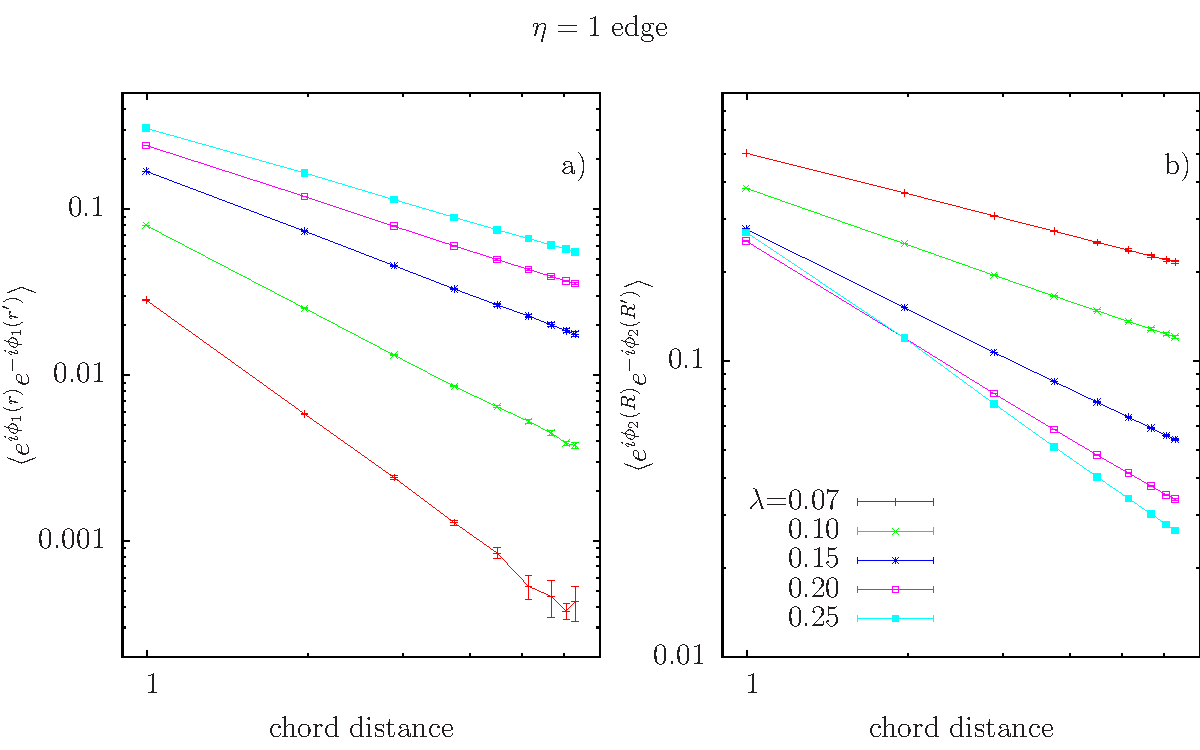
\includegraphics[width=\linewidth]{figures/onecord.eps}
\caption{ Correlation functions a) $\chi_1$ and b) $\chi_2$, plotted against the chord distance of Eq.~(\ref{cordlength}), on a log-log scale, for $\eta=1$ edge.  Error bars come from comparing runs with different initial conditions.  The straight lines imply that we have algebraic decay in the correlation functions and therefore the edge is gapless.  The slope of these lines varies with $\lambda$, and the extracted exponents are shown in Fig.~\ref{exponents}.}
\label{onegood}
\end{figure}

Figure \ref{twogood} shows the same measurements for $\eta=2$. Again we see evidence of algebraic decay with exponents which depend on $\lambda$. As above, we used the reformulation in Eq.~(\ref{Sint}) for the $\chi_2$ measurements. Note that for this data it is important to measure correlators of $\exp(i2\phi_2)$, as defined in Eq.~(\ref{Crr}). As expected, we found that single-boson correlators decay exponentially in this case, and only pair-boson correlators show algebraic decay.


From the above data we can extract the exponents of the algebraic decay. We fit the above data to the function
\begin{equation}
\chi_1(r-r')=\frac{A}{\left[\frac{L}{\pi}\sin\left(\frac{\pi|r-r'|}{L}\right)\right]^{b_{\chi_1}}},
\label{fitfunction}
\end{equation}
with $A$ and $b_{\chi_1}$ parameters of the fit. We analyzed $\chi_2$ similarly.  Figure~\ref{exponents} shows plots of these exponents for $\eta=1$ and $\eta=2$. The decay exponents for both $\chi_1$ and $\chi_2$ are slightly above the spin-wave prediction at small $\lambda$ (e.g., within 10\% for $\lambda =0.07$). At large $\lambda$ the fitted exponents differ significantly from the naive spin-wave predictions, though within an order of magnitude. In Appendix \ref{app:connections} we discuss a phenomenological understanding of the edge which predicts that the product of these exponents in the integer quantum Hall case should be equal to $1$. We can see from Fig.~\ref{exponents} that the products we measured are approximately equal to one.

\begin{figure}
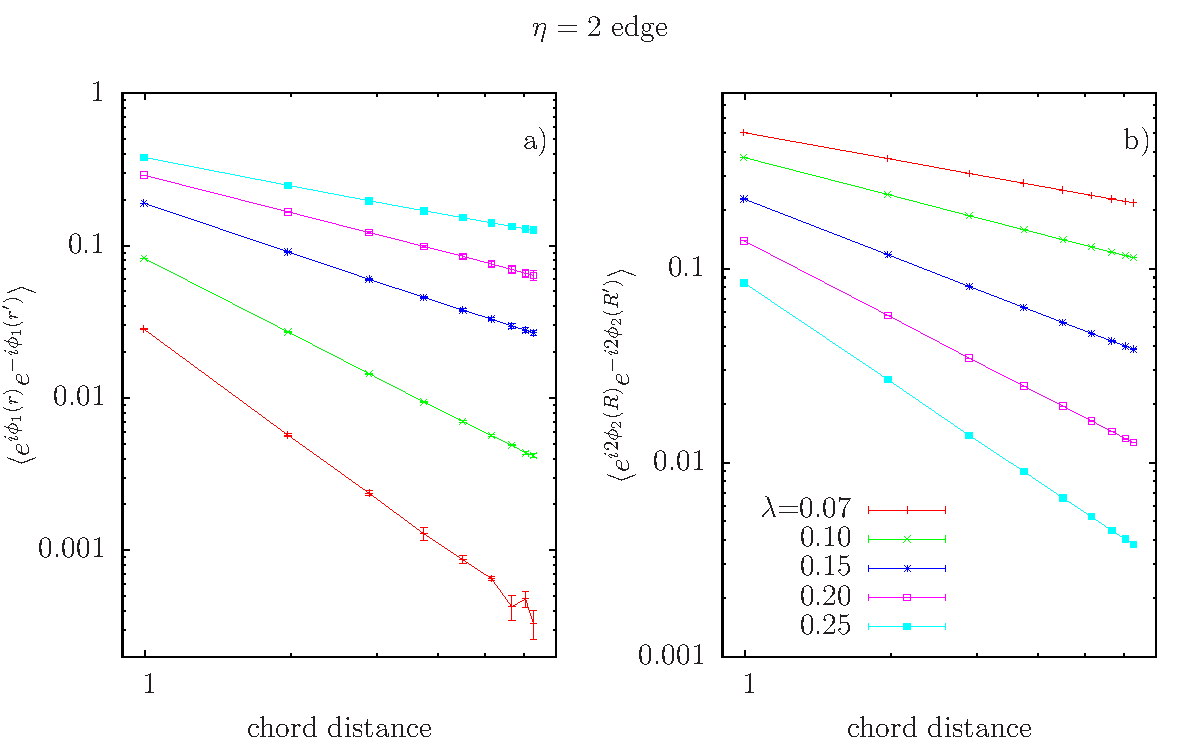
\includegraphics[width=\linewidth]{figures/twocord.eps}
\caption{ Same as Fig.~\ref{onegood}, but for $\eta=2$ edge. Once again, we see evidence for gapless modes. Note that in b) we measure pair-boson $e^{i 2\phi_2}$ correlators on the edge, while single-boson $e^{i\phi_2}$ correlators decay exponentially.
\label{twogood}}
\end{figure}

\begin{figure}
\includegraphics[width=0.6\linewidth,angle=-90]{figures/exp1.eps}
\caption{ The exponents of the algebraic decay for $\eta=1$ and $\eta=2$, extracted using the fitting function in Eq.~(\ref{fitfunction}). We see that the $b_{\chi_1}$ exponent decreases with increasing $\lambda$ while the $b_{\chi_2}$ exponent increases. The product of these exponents is also shown.
\label{exponents}}
\end{figure}

Figure~\ref{onethird} shows $\chi_2$ for $\eta=1/3$. The existence of straight lines in this plot implies that we have gapless modes in a fractional quantum Hall system. We acquired this data using the reformulation in Eq.~(\ref{Sfrac2}). We were unable to measure $\chi_1$ for the fractional cases because the decay exponents were too large. Recall that in order to have gapped $\cal{G}$ variables we need $\lambda d^2 \lesssim 0.33$; for $d^2=9$ this leads to a small $\lambda$, and the spin-wave theory estimate Eq.~(\ref{bchi1_sw}) tells us that this leads to large exponents for $\chi_1$.  The presence of the factor $d^2$ in the product $b_{\chi_1} b_{\chi_2} \approx d^2$, which we obtained here by the direct analysis, is an indirect manifestation of the fractionalization when parameter $d>1$.  Indeed, in Appendix~\ref{app:connections} we use phenomenological model of the edge and the fractionalization of the particles to show that the product of these exponents should be equal to $d^2$, while if there is no fractionalization the product will be equal to $1$. In our lattice model of the edge and the specific parameterizations of the potentials, we have found that the values of $b_{\chi_2}$ are numerically similar to those in the integer case, but the $b_{\chi_1}$ values are much larger. This implies that the product of the exponents is greater than $1$, providing indirect evidence for fractionalization.

\begin{figure}
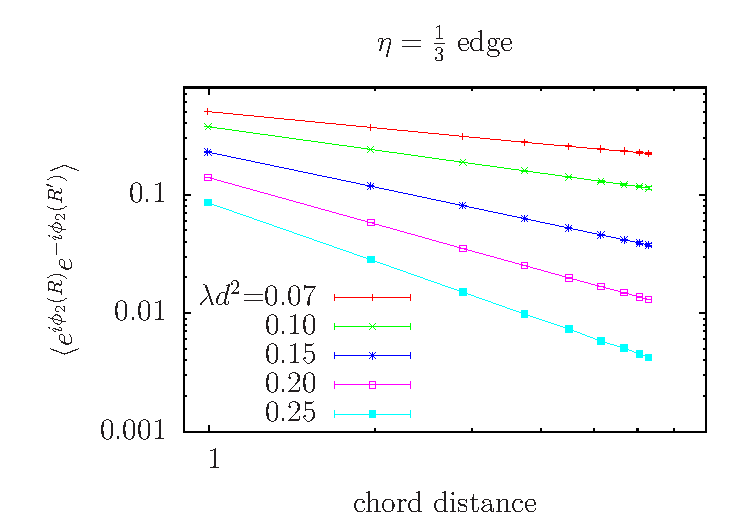
\includegraphics[width=\linewidth]{figures/thirdcord.eps}
\caption{ $\chi_2$ correlation function for $\eta=1/3$ edge, where $c=1$, $d=3$. The straight lines indicate algebraic decay for this fractional case. We were unable to obtain data for $\chi_1$ because it decayed too quickly.
\label{onethird}}
\end{figure}


%%%%%%%%%%%%%%%%%%%%%%%%%%%%%%%%%%%%%%%%%%%%%%%%%%%%%%%%%%%%%%%%%%%%%%%%%
\section{Phase diagrams}
\label{sec:reverse}

In previous works\cite{Loopy,short_range3,Gen2Loops} we have studied actions similar to that in Eq.~(\ref{kaction_2}). However, in those works we considered only the case where $\theta(k)$ was equal to a rational constant multiplied by $2\pi$. These are precisely the actions of the $\GG$ variables which appeared in Eq.~(\ref{gaction}), and from now on we will refer to them as ``statistical'' actions. The statistical variables are quasiparticles in the quantum Hall phases.  In Refs.~\cite{Loopy, short_range3} we did not attempt to connect the statistical actions to a physical system, and instead focused on their phase diagrams.  Therefore we did not specify the ``vacuum'' of physical variables as it does not affect the dynamics of the phase transitions, but it is this vacuum which carries the quantized $\sigma^{12}_{xy}$ as can be seen from Eq.~(\ref{gaction}).  Furthermore, we can now also specify physical charges of the quasiparticles.  

If we start with a statistical action with rational $\theta_{\cG}$, we can invert the change of variables procedure in Sec.~(\ref{sec::demon}) with the correct choice of $a,b,c,d$ to get an action with $\theta(k)\sim k^2$, as in Eq.~(\ref{action}), which we will from now on call the ``physical'' action. This is how we obtained the specific potentials in Eqs.~(\ref{vintro}) and (\ref{tintro}). We know from the previous works the phase diagrams of the statistical actions in terms of the variables $\GG$. We can use the change of variables in this work to describe these phase diagrams in terms of the physical variables $\JJ$. 

Recall that the specific potentials can be classified by the coefficients $c$ and $d$. When changing from the physical variables $\JJ$ to the statistical variables $\GG$, we need these coefficients as well as $a$ and $b$, but these coefficients are not independent since they must satisfy $ad-bc=1$. In particular, if we have one solution $a_0$, $b_0$ then this constraint tells us that 
\begin{eqnarray}
&&a=a_0 + mc,\nonumber\\
&&b=b_0 + md,
\label{bshift} 
\end{eqnarray} 
are also solutions if $m$ is an integer.  The statistical actions can be classified by their statistical angle, which for our specific potential choices is given by $\theta_\cG=2\pi b/d$. Therefore each physical action can be related to multiple statistical actions by our change of variables. However, these statistical actions differ only in that $\theta_\cG$ can be different by an integer multiple of $2\pi$. Such a shift will have no effect on the partition sum in the $\GG$ variables. Therefore all of the statistical actions which can be related to a given physical action have the same behavior. 

We can also see that multiple physical actions whose ratio $c/d$ differ by an integer can also be mapped to the same statistical action: that is, the actions in terms of $\cal{G}$ particles are essentially the same except for the ``background'' quantum Hall conductivity $\sigma^{12}_{xy}$ changing by an even integer. These physical actions are related to each other by adding an ``integer quantum Hall layer'' to the system without changing the properties of the fractionalized excitations. 

To begin the discussion of the broader phase diagrams of our models, it is useful to consider also the action in terms of the dual variables $\QQ_1$, $\QQ_2$:
\begin{eqnarray}
S &=& \frac{1}{2}\sum_k \frac{(2\pi)^2 }{|\vec{f}_k|^2} \left[\lambda_1|\QQ_1(k)|^2+\lambda_2|\QQ_2(k)|^2\right]\nonumber\\
&+& i\sum_k \frac{2\pi c}{d} \QQ_1(-k)\cdot \vec{a}_{\QQ2}(k),
\label{qaction}
\end{eqnarray}
where $\QQ_2=\curl\vec{a}_{\QQ2}$. This action comes from dualizing the $\cJ_1$, $\cJ_2$ variables with the specific potentials in Eqs.~(\ref{vintro}) and (\ref{tintro}). [Eq.~(15) in Ref.~\cite{short_range3} contains this action with general potentials.] This action can also be obtained by applying the modular transformation $(0, -1, 1, 0)$ to the original action. Note that the $d$ in Eq.~(\ref{qaction}) corresponds to the parameter in Eqs.~(\ref{vintro})-(\ref{tintro}), and is not related to the modular transformation used to obtain this phase.  The $\cQ$ variables are vortices with the usual long-range intra-species interactions, $v_{\cQ}(k) \sim 1/k^2$ in momentum space, and we see that these vortices are gapped for large $\lambda_1$ and $\lambda_2$.  The statistical angle in the third term of Eq.~(\ref{qaction}) is a rational number.  However, this rational number is unique to the specific choices we made in Eqs.~(\ref{vintro})-(\ref{tintro}), and small short-range modifications of the model can lead to a different statistical angle for the $\QQ$ variables.  This is unlike the rational $\theta_{\GG}$ in the quantum Hall insulators which is robust to short-range modifications of the potentials.  The difference comes from the qualitative difference when applying Eq.~(\ref{VJ}) to generic short-ranged $v(k) \sim {\rm const}$ and $\theta(k) \sim k^2$ in the cases $d=0$ (duality to only vortices) and $d\neq 0$ (more general modular transformation).

\subsection{Models with $c/d=n$, $\sigma^{12}_{xy}=2n$}
We now turn to detailed descriptions of the phase diagrams.
First we discuss the case where the conductivity in the quantum Hall phase is quantized as an even integer. In this case we start with a physical action with the potentials Eqs.~(\ref{vintro})-(\ref{tintro}) with parameters $c=n$, $d=1$ for $n$ an integer. We can get a statistical action by applying the modular transformation $(1, 0, n, 1)$, and this gives a statistical action with $\theta_{\GG}=0$ and a background Hall conductivity of $\sigma^{12}_{xy}=2n$. Therefore in the statistical action we have a system of  two uncoupled loops, which is a system that is well understood.\cite{Cha1991,Sorensen} 
In this system when $\lambda_i\lesssim 0.3325$, the variables $\GG_i$ are gapped, and when $\lambda_i$ is greater than this value the $\GG_i$ are condensed. All phase transitions are second-order XY transitions. Figure \ref{intphase} shows this phase diagram. 
Since we know the behavior of the $\GG$ variables everywhere in the phase diagram, we can now deduce the behavior of the physical $\JJ$ variables. In the lower left corner phase we have seen that the $\JJ$ variables are in a quantum Hall phase. 

To understand the rest of the phase diagram we must make more precise our earlier definitions of what makes a variable ``gapped'' or ``condensed''. When a variable is in a phase in which it is gapped, the energy cost for having large loops of that variable becomes arbitrarily large and only small loops are present. When a variable is condensed the energy cost for forming loops is small. A variable is condensed if and only if the variable dual to it is gapped. In some phases a variable will be neither condensed nor gapped in the above sense; instead the variable can be part of a composite object which is condensed or gapped. This is the situation for the $\cJ$ variables in the quantum Hall phases. We bring this out to indicate that there are more cases than just given by binary choice of $\cJ_i$ variable being gapped or condensed.  In all cases, the precise meaning is provided by finding appropriate transformation that leads to a description in terms of gapped particles only.

With this in mind, we can interpret the rest of the phase diagram. We begin with the phase in the upper-right corner, where $\lambda_1$ and $\lambda_2$ are large. We can see that in this phase the potentials seen by the $\QQ$ variables in Eq.~(\ref{qaction}) become arbitrarily large, so both of these species of variable are gapped. Therefore both species of $\JJ$ variable are condensed and this phase is a superfluid. The conductivities $\sigma^{11}_{xx}$ and $\sigma^{22}_{xx}$ diverge in this phase, while the Hall conductivity $\sigma^{12}_{xy}$ is non-universal. 

We now study the off-diagonal phases in Fig.~\ref{intphase}. For simplicity we discuss the phase in the lower right corner where $\lambda_1$ is large but $\lambda_2$ is small (in fact $\lambda_1$ can become arbitrarily large in this phase). The upper left corner is similar with the indices interchanged. From Eq.~(\ref{vintro}) we can see that when $\lambda_1\rightarrow\infty$,  $v_2(k)\rightarrow\frac{1}{\lambda_2}$. Since $\lambda_2$ is small in this phase, $v_2(k)$ can become arbitrarily large and the $\JJ_2$ variables must be gapped. In addition, we can see from Eq.~(\ref{JQreal}) that the $\QQ_1$ variables see an arbitrarily large potential and are therefore gapped, so the $\JJ_1$ variables are condensed. From the above results, we can conclude that this phase is a trivial insulator in the $\JJ_2$ variables and a superfluid in the $\JJ_1$ variables.

\begin{figure}
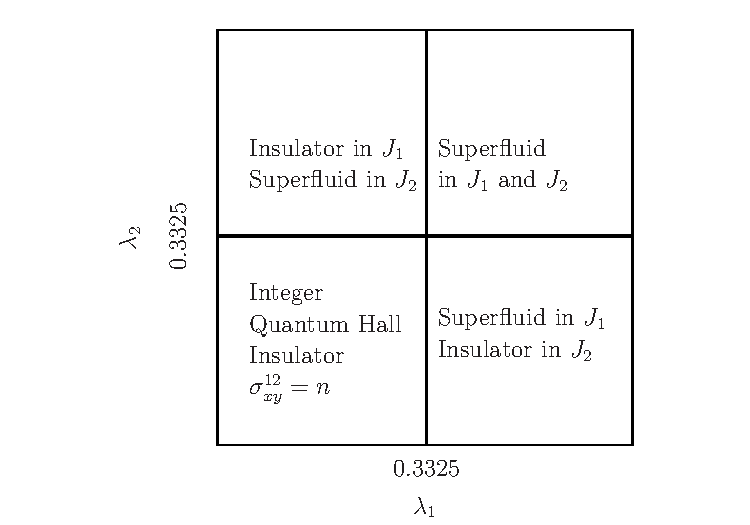
\includegraphics[width=\linewidth]{figures/intphase.eps}
\caption{The phase diagram for the model with the potentials of Eqs.~(\ref{vintro})-(\ref{tintro}) and $c=n$, $d=1$. In the lower left phase the $\GG$ variables are gapped and we have the integer quantum Hall phase with $\sigma^{12}_{xy}=2n$. In the upper right phase the $\JJ$ variables are condensed, and we have a superfluid.  In the off-diagonal phases, one of the $\cJ$ variables is condensed and the other is gapped.}
\label{intphase}
\end{figure}

Finally, we note that the specific model, Eqs.~(\ref{vintro})-(\ref{tintro}), with $c=n, d=1$ does not realize the trivial insulator phase with both $\cJ_1$ and $\cJ_2$ gapped.  Of course, we can obtain such a phase by different modifications of the potentials, e.g., by adding large repulsive pieces to both $v_1$ and $v_2$, and it would be interesting to study such models in the future.


%%%%%%%%%%%%%%%%%%%%%%%%%%%%%%%%%%%%%%%%%%%%%%%%%%%%%%%%%%%%%%%%%%%%%%%%
\subsection{Models with $d\neq 1$}
In Ref.~\cite{short_range3} we studied a statistical action with $\theta_{\cal{G}} = 2\pi/3$. The phase diagram for this model is shown in Fig.~\ref{fracphase}. In the lower left corner the $\GG$ variables are gapped and this is the fractional quantum Hall phase. Any physical action with $d=3$ and $c=1+3m$ (for $m$ an integer) can be related to this statistical action by our modular transformation; here we will discuss the case where $c=1$. In this case the change of variables needed to get from the $\JJ$ variables to the $\GG$ variables is $(0, -1, 1, 3)$. The fractional quantum Hall phase will have $\sigma^{12}_{xy}=2\cdot\frac{1}{3}$ and excitations carrying respective fractional charges of $1/3$ and mutual statistics of $2\pi/3$.

We know from our previous numerical study\cite{short_range3} that in the middle phase the variables dual to the $\GG$ variables are gapped. 
We can also compute the action for the variables dual to the $\GG$ variables and see that it has the same potential as the action for the $\JJ$ variables. The two actions also have values of $\theta(k)$ which differ only by an integer multiple of $2\pi$. Such difference will translate to factors $e^{2\pi i}$ in the partition sum and therefore will not contribute. Therefore if the variables dual to the $\GG$ variables are gapped then the $\JJ$ variables should also be gapped. Therefore this middle phase is a trivial insulator in the $\JJ$ variables. This can be confirmed by measuring the conductivity numerically in this phase. 

In the upper right corner phase we can see from Eq.~(\ref{qaction}) that the $\cQ$ variables are gapped,  and therefore the $\JJ$ variables are condensed and this phase is a superfluid.  In our previous work\cite{short_range3} we found that transition between the trivial insulator and the superfluid is a pair of XY transitions, while we found more complicated behavior at the fractional quantum Hall-trivial insulator transition. 

The structure described in the previous paragraph holds for any set of physical variables which can be mapped to a statistical action with $\theta_\cG=2\pi/m$, with $m$ an integer. %\cite{footnoten2}.
One exception is $m=2$, where our specific model with $c=1, d=2$ has an additional symmetry in the $\cG$ variables which prevents the existence of the middle phase, cf.~Fig.~1 in Ref.~\cite{Loopy}.  This is discussed in detail in Refs.~\cite{Loopy, Gen2Loops}, while here we note that generic perturbations to our original model will break this symmetry and open a sliver of the trivial phase in the phase diagram.

Finally, for more complicated fractions $c/d$, our model will have multiple phases in the middle of the phase diagram, resembling hierarchy of phases that we found in $U(1) \times U(1)$ loop models with marginally long-ranged interactions and modular invariance.\cite{Gen2Loops}  We expect that the ``middle'' phase at the largest $\lambda$ is a trivial insulator, while the other phases are various quantum Hall states.  For example, in our model Eqs.~(\ref{vintro})-(\ref{tintro}) with $c=2, d=5$, we found the following sequence of phases upon increasing $\lambda_1 = \lambda_2$: fractional quantum Hall insulators $\sigma^{12}_{xy} = 2\cdot 2/5$ and $\sigma^{12}_{xy} = 2\cdot 1/2$, trivial insulator $\sigma^{12}_{xy} = 0$, and superfluid.  It would be interesting to explore such phase diagrams and phase transitions in more detail in the future.

\begin{figure}
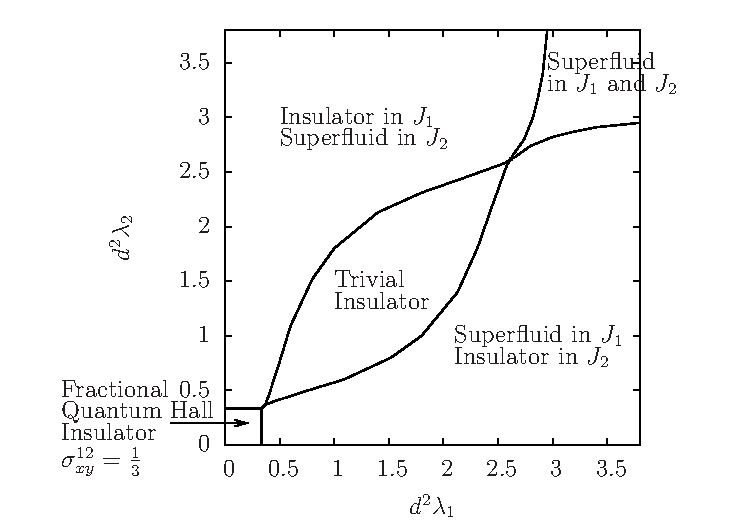
\includegraphics[width=\linewidth]{figures/fracphase.eps}
\caption{The phase diagram for the model with $c=1,d=3$. In the lower left phase the $\GG$ variables are gapped and we have a fractional quantum Hall phase with $\sigma^{12}_{xy}=2\cdot\frac{1}{3}$. In the upper right phase the $\JJ$ variables are condensed, which implies a superfluid. In the middle phase the $\JJ$ variables are gapped and we have a trivial insulator. This figure is reproduced from Ref.~\cite{short_range3}, but the phases have been re-interpreted in terms of the physical variables discussed in this work.}
\label{fracphase}
\end{figure}


%%%%%%%%%%%%%%%%%%%%%%%%%%%%%%%%%%%%%%%%%%%%%%%%%%%%%%%%%%%%%%%%%%
\section{Hamiltonian formulation}
\label{app:H}
Throughout the main text, we worked with the Euclidean action formulation of the model.  The action for the physical currents is local in (2+1)D space-time and is very convenient for analysis.  However, it is natural to ask whether this action can be realized as a path integral of a local Hamiltonian in 2d.\cite{Matthew_Alexei_thanks}  Below we provide an example of such a Hamiltonian.

We first specify the physical Hilbert space.  Our degrees of freedom reside on two inter-penetrating square lattices as shown in Fig.~\ref{fig:H}.  We place quantum U(1) rotors on sites $\br$ of the first square lattice.  The rotors are described by $2\pi$-periodic phase variables $\hat{\phi}_1(\br)$ and conjugate integer number variables $\hat{n}_1(\br)$, with commutation relations $[\hat{\phi}_1(\br), \hat{n}_1(\br')] = i \delta_{\br\br'}$.  We place another set of U(1) rotors, described by $\hat{\phi}_2(\bR)$ and $\hat{n}_2(\bR)$, on sites $\bR$ of the second (dual) square lattice.  Finally, we place harmonic oscillators, described by $\hat{\chi}_\ell$ and $\hat{\pi}_\ell$, on centers of links of the first square lattice, which are also centers of links of the second square lattice, e.g., $\ell = <\br, \br + \hat{\bx}> = <\bR, \bR + \hat{\by}>$ as illustrated in Fig.~\ref{fig:H}.  Here $\hat{\chi}_\ell$ are real-valued coordinate variables and $\hat{\pi}_\ell$ are conjugate momentum variables, $[\hat{\chi}_\ell, \hat{\pi}_{\ell'}] = i\delta_{\ell\ell'}$.  Looking ahead, we will use a path integral containing both $\chi_\ell$ and $\pi_\ell$.  We will view the coordinate variables as fields on the links of the first lattice,
\begin{equation}
\hat{\alpha}_{1j}(\br) \equiv \hat{\chi}_{\br, \br + \hat{\bj}} ~,
\end{equation}
$\hat{\bj} = \hat{\bx}$ or $\hat{\by}$, while we will view the conjugate momentum variables as fields on the links of the second lattice,
\begin{equation}
\hat{\alpha}_{2j}(\bR) = \epsilon_{jk} \hat{\pi}_{\br, \br + \hat{\bk}} ~.
\end{equation}
Here $\epsilon_{xy} = -\epsilon_{yx} = 1$ is the 2d antisymmetric tensor and $<\bR, \bR + \hat{\bj}>$ and $<\br, \br + \hat{\bk}>$ are crossing links.\cite{footnoteKitaev}
Note that in this Appendix we adopt the following notation:  Spatial lattice sites are labeled with bold face, e.g., $\br, \bR$.  Spatial directions are labeled with Roman letters, e.g., $j, k$; space-time directions that appear later will be labeled with Greek letters, e.g., $\mu, \nu$.  Oriented fields residing on spatial links are viewed as spatial vectors and are labeled with bold face, e.g., ${\bm \alpha_1}, {\bm \alpha_2}$.

%\begin{figure}[t!]
%\input{H.pstex_t}
%\caption{Our Hamiltonian Eq.~(\ref{H}) has U(1) rotors residing on sites $\br$ of the direct square lattice and U(1) rotors residing on sites $\bR$ of the dual lattice.  We also have harmonic oscillators residing on crosses $\ell$ of the links of the two lattices.  The first and second U(1) systems are coupled to the oscillator position and momentum variables respectively as if the latter were gauge fields.\cite{footnoteKitaev}  With appropriate choices of parameters and additional charge-flux couplings, we can induce condensations of bound states of charges and vortices leading to the quantum Hall states discussed in the main text.}
%\label{fig:H}
%\end{figure}


Our Hamiltonian is:
\begin{eqnarray}
\label{H}
\hat{H} &=& \hat{H}_{h1} + \hat{H}_{h2} + \hat{H}_{u1} + \hat{H}_{u2} + \hat{H}_\chi + \hat{H}_\pi ~,\\
\hat{H}_{h1} &=& -\sum_{\br, j} h_1 \cos[\nabla_j \hat{\phi}_1(\br) - e_1 \hat{\alpha}_{1j}(\br)] ~,\\
\hat{H}_{h2} &=& -\sum_{\bR, j} h_2 \cos[\nabla_j \hat{\phi}_2(\bR) - e_2 \hat{\alpha}_{2j}(\bR)] ~,\\
\hat{H}_{u1} &=& \frac{1}{2} \sum_\br u_1 \left[\hat{n}_1(\br) + g_1 ({\bm \nabla} \wedge \hat{\bm \alpha}_2)(\br) \right]^2 ~,\\
\hat{H}_{u2} &=& \frac{1}{2} \sum_\bR u_2 \left[\hat{n}_2(\bR) + g_2 ({\bm \nabla} \wedge \hat{\bm \alpha}_1)(\bR) \right]^2 ~,\\
\hat{H}_\chi &=& \sum_\ell \frac{\kappa\, \hat{\chi}_\ell^2}{2} ~, \quad
\hat{H}_\pi = \sum_\ell \frac{\hat{\pi}_\ell^2}{2m} ~.
\end{eqnarray}
Here we introduced various parameters such as boson hopping amplitudes $h_1$ and $h_2$, on-site energies $u_1$ and $u_2$, and oscillator parameters $\kappa$ and $m$.  The hopping terms couple the boson phases and the oscillators as if the latter were ``gauge fields.''  The on-site terms couple the boson numbers and appropriate fluxes of the ``gauge fields'': e.g., flux ${\bm \nabla} \wedge \hat{\bm \alpha}_1 \equiv \nabla_x \hat{\alpha}_{1y} - \nabla_y \hat{\alpha}_{1x}$ is associated with a plaquette of the first lattice, or, equivalently a site $\bR$ of the dual lattice, and is coupled with the boson number $\hat{n}_2(\bR)$ on that site.  The corresponding parameters $e_1, e_2, g_1, g_2$ will be chosen later. 
Here we emphasize that the model is local in the physical variables (i.e., it is not a gauge theory), in the same spirit as Kitaev's toric code model.

We develop imaginary-time path integral by using Trotter decomposition and insertions of unity as follows:
\begin{eqnarray*}
e^{-\delta\tau \hat{H}} &\approx& e^{-\delta\tau (\hat{H}_{u1} + \hat{H}_{h2} + \hat{H}_\pi)} e^{-\delta\tau (\hat{H}_{h1} + \hat{H}_{u2} + \hat{H}_\chi)}
= ~\mathbbm{1}_{\tau + \delta\tau}~ e^{-\delta\tau (\hat{H}_{u1} + \hat{H}_{h2} + \hat{H}_\pi)} ~\mathbbm{1}_{\tau + \frac{\delta\tau}{2}}~ e^{-\delta\tau (\hat{H}_{h1} + \hat{H}_{u2} + \hat{H}_\chi)} ~\mathbbm{1}_{\tau} ~,\\
\mathbbm{1}_{\tau} &=&
\int_{-\pi}^\pi D\phi_1(\br, \tau)
\sum_{n_2(\bR, \tau) = -\infty}^\infty
\int_{-\infty}^\infty D\chi_\ell(\tau) ~
\Big|   \phi_1(\br, \tau), n_2(\bR, \tau), \chi_\ell(\tau) \Big\ra
\Big\la \phi_1(\br, \tau), n_2(\bR, \tau), \chi_\ell(\tau) \Big| ~,\\
\mathbbm{1}_{\tau_\half \equiv \tau + \frac{\delta\tau}{2}} &=&
\sum_{n_1(\br, \tau_\half) = -\infty}^\infty
\int_{-\pi}^\pi D\phi_2(\bR, \tau_\half) 
\int_{-\infty}^\infty D\pi_\ell(\tau_\half) ~
\Big|   n_1(\br, \tau_\half), \phi_2(\bR, \tau_\half), \pi_\ell(\tau_\half) \Big\ra
\Big\la n_1(\br, \tau_\half), \phi_2(\bR, \tau_\half), \pi_\ell(\tau_\half) \Big| ~.
\end{eqnarray*}
Here we used one set of variables on ``integer'' time slices $\tau = {\rm int} \times \delta\tau$ and conjugate variables on ``half-integer'' time slices $\tau_\half \equiv \tau + \delta\tau/2$.  We also arranged the Trotter decomposition so that the pieces of the Hamiltonian act as $c$-numbers on the kets of the above insertions of unity.  Throughout, we omit normalization constants.  The remaining inputs to complete the path integral formulation in the above variables are overlaps such as
\begin{eqnarray}
\big\la \chi_\ell(\tau + \delta\tau) \big| \pi_\ell(\tau_\half) \big\ra
\big\la \pi_\ell(\tau_\half) \big| \chi_\ell(\tau) \big\ra &=& e^{i \pi_\ell(\tau_\half) [\chi_\ell(\tau + \delta\tau) - \chi_\ell(\tau)]}
= e^{i \alpha_{2k} \epsilon_{kj} \nabla_\tau \alpha_{1j}} ~,
\quad {\rm for~} \ell = <\br, \br+\hat{\bj}>, ~ \\
\big\la \phi_1(\br, \tau + \delta\tau) \big| n_1(\br, \tau_\half) \big\ra
\big\la n_1(\br, \tau_\half) \big| \phi_1(\br, \tau) \big\ra &=&
e^{i n_1(\br, \tau_\half) [\phi_1(\br, \tau + \delta\tau) - \phi_1(\br, \tau)]}
= e^{i \cJ_{1\tau} \nabla_\tau \phi_1} ~,
\end{eqnarray}
ans similarly for the second rotor variables.

In the action, we have phase variables $\phi_1(\br, \tau)$ residing on sites $(\br, \tau)$ of a (2+1)D cubic lattice and $\phi_2(\bR, \tau_\half)$ residing on sites $(\bR, \tau_\half)$ of a dual cubic lattice (in the main text, such space-time points are labeled simply $r$ and $R$).  We also have boson number variables $n_1(\br, \tau_\half)$ and $n_2(\bR, \tau)$, which we can view as residing on temporal links of the first and second (dual) cubic lattices respectively and write as temporal components of boson three-currents, $\cJ_{1\tau}(\br, \tau) \equiv n_1(\br, \tau_\half)$ and $\cJ_{2\tau}(\bR, \tau_\half) \equiv n_2(\bR, \tau + \delta\tau)$.  We introduce spatial current components using an approach familiar in treatments of XY models; namely, we interpret the cosine terms in $\hat{H}_{h1}$ and $\hat{H}_{h2}$ as so-called Villain cosines and write, e.g.,
\begin{eqnarray*}
&& e^{\delta\tau h_1 \cos[\nabla_j \phi_1(\br, \tau) - e_1 \alpha_{1j}(\br, \tau)]} \\
&& \to \sum_{\cJ_{1j}(\br, \tau) = -\infty}^\infty e^{-\frac{\cJ_{1j}^2}{2 \delta\tau h_1} + i \cJ_{1j} [\nabla_j \phi_1 - e_1 \alpha_{1j}]} ~.
\end{eqnarray*}
We can now integrate over the phase degrees of freedom and obtain current conservation conditions, $\vec{\nabla} \cdot \vcJ_1 \equiv \sum_{\mu=x, y, \tau} \nabla_\mu \cJ_{1\mu} = 0$, and similarly for the three-current $\vcJ_2$.
Here and below, arrows over symbols denote three-vectors such as $\vcJ_1 = (\cJ_{1x}, \cJ_{1y}, \cJ_{1\tau})$, while bold symbols refer to spatial parts such as ${\bm \cJ}_1 = (\cJ_{1x}, \cJ_{1y})$.

We still have the oscillator variables, now labeled ${\bm \alpha}_1(\br, \tau)$ and ${\bm \alpha}_2(\bR, \tau_\half)$ and residing on spatial links of the first and second cubic lattices.  At this point, we could also integrate over these variables and obtain an action in terms of the boson three-currents only.  To facilitate the integration and show the connection with the loop models in the main text, we will first write the on-site terms by introducing auxiliary fields labeled $\alpha_{1\tau}$ and $\alpha_{2\tau}$ residing on the temporal links of the first and second cubic lattices respectively, e.g.:
\begin{eqnarray*}
&& e^{-\frac{\delta\tau u_2}{2} \left[\cJ_{2\tau}(\bR, \tau_\half) + g_2 ({\bm \nabla} \wedge {\bm \alpha}_1)(\bR, \tau_\half) \right]^2} \\
&& = \int_{-\infty}^\infty d\alpha_{2\tau}(\bR, \tau_\half) e^{-\frac{\alpha_{2\tau}^2}{2 \delta\tau u_2} - i \alpha_{2\tau} \left[J_{2\tau} + g_2 ({\bm \nabla} \wedge {\bm \alpha}_1) \right]} ~.
\end{eqnarray*}
For brevity, we often omit the lattice coordinates on the fields and imply precise geometric relation between objects on different lattices: e.g., an oriented plaquette on one lattice is also associated with a unique oriented bond on the other lattice crossing this plaquette.

Putting everything together, the final action takes the form
\begin{eqnarray*}
&& S[\valpha_1, \valpha_2, \vcJ_1, \vcJ_2] = 
\sum \left[ \frac{\delta\tau \kappa\, {\bm \alpha}_1^2}{2} + \frac{\alpha_{1\tau}^2}{2\delta\tau u_1} + \frac{\delta\tau {\bm \alpha}_2^2}{2m} + \frac{\alpha_{2\tau}^2}{2\delta\tau u_2} \right]
+ \sum \left[\frac{{\bm \cJ}_1^2}{2\delta\tau h_1} + \frac{{\bm \cJ}_2^2}{2\delta\tau h_2} \right] \\
&&\quad + i \sum \left[ (\nabla_\tau{\bm \alpha}_1) \wedge {\bm \alpha}_2 + g_1 \alpha_{1\tau} ({\bm \nabla} \wedge {\bm \alpha}_2) + g_2 \alpha_{2\tau} ({\bm \nabla} \wedge {\bm \alpha}_1) \right]
+ i \sum \left[ e_1 {\bm \cJ}_1 \cdot {\bm \alpha}_1 + \cJ_{1\tau} \alpha_{1\tau} + e_2 {\bm \cJ}_2 \cdot {\bm \alpha}_2 + \cJ_{2\tau} \alpha_{2\tau} \right] ~. 
\end{eqnarray*}
Here the wedge operator is ${\bm v}_1 \wedge {\bm v}_2 \equiv \sum_{j,k} \epsilon_{jk} v_{1j} v_{2k} = v_{1x} v_{2y} - v_{1y} v_{2x}$.
By rescaling ${\bm \alpha}_1 = {\bm \alpha}^\prime_1/e_1$ and similarly for  ${\bm \alpha}_2$, and choosing, e.g., $e_1 = e_2 = 1/g_1 = 1/g_2 = \sqrt{2\pi d/c}$, we obtain essentially the same action as in Eq.~(\ref{preal}) in the main text.  The only difference from the main text is that there are additional local current interactions containing $h_1$ and $h_2$ couplings, and to make the actions identical we only need to take $h_1$ and $h_2$ large.  In particular, the model is in the ``$c/d$'' Quantum Hall phase for sufficiently small $\kappa$ and sufficiently large $m$ and large $u_1, u_2$.
Thus, we have provided a Hamiltonian realization for our Quantum Hall phases.

We can also carry out this derivation when the parameters $h_{1,2}, u_{1,2}, \kappa, m, e_{1,2}, g_{1,2}$ vary in space; in particular, we can study a boundary between Quantum Hall and trivial insulators.
Note that there is significant freedom in how to vary the parameters to achieve different phases even within the specific model.  For example, we can obtain a trivial insulator by taking $e_{1,2}$ and $g_{1,2}$ to be zero while also taking the hopping amplitudes $h_{1,2}$ to be small and on-site potentials $u_{1,2}$ large.
Alternatively, we can take $e_{1,2}$ to be very large while $g_{1,2} \to 0$ and can reach the trivial insulator this way even when the bare hopping amplitudes $h_{1,2}$ are large (in this case, the boson propagation is scrambled by strong phase coupling to the oscillators).  The latter route is closer to the model we used in the main text when discussing a boundary between Quantum Hall and trivial insulators.  Such a boundary model in the present Hamiltonian approach will in general differ from that in the main text.  Indeed, in the Chern-Simons-like piece for the rescaled $\valpha^\prime_{1,2}$ variables,
\begin{equation*}
i \sum [ \frac{(\nabla_\tau {\bm \alpha}^\prime_1) \wedge {\bm \alpha}^\prime_2}{e_1 e_2} + g_1 \alpha_{1\tau} ({\bm \nabla} \wedge \frac{{\bm \alpha}^\prime_2}{e_2}) + g_2 \alpha_{2\tau} ({\bm \nabla} \wedge \frac{{\bm \alpha}^\prime_1}{e_1}) ] ~,
\end{equation*}
the spatially varying $e$ and $g$ couplings can appear non-trivially under spatial derivatives, and the action in general cannot be cast in the form of Eq.~(\ref{JQreal}).  However, we can find a pattern of couplings that will reproduce our boundary model in the main text:  If we take $1/e_a = g_a = \sqrt{c/(2\pi d)}$ for $x\in [x_{aL}, x_{aR}]$ and $1/e_a = g_a = 0$ otherwise, and take the region $[x_{2L}, x_{2R}]$ to be inside the region $[x_{1L}, x_{1R}]$, we eliminate terms with non-desired derivatives of the couplings and can recast the Chern-Simons-like piece for the rescaled $\valpha^\prime_{1,2}$ variables into the form of Eq.~(\ref{JQreal}) with $\eta(R) = c/d$ inside $[x_{2L}, x_{2R}]$ and zero outside.  Thus, we have also provided a Hamiltonian realization of the boundary model used in the main text.

While we universally expect gapless boson correlations on the boundary, detailed aspects can be different for different realizations.  In this paper, we have focused on the crude demonstration of the gaplessness for the specific boundary model in the main text.  In future work, it would be interesting to examine different realizations and systematically explore all aspects of possible edge theories.

%%%%%%%%%%%%%%%%%%%%%%%%%%%%%%%%%%%%%%%%%%%%%%%%%%%%%%%%%%%%%%%%%%%%%%%%
\section{Discussion}
In this work we have presented physical $U(1) \times U(1)$ bosonic models which realize insulating phases with a quantized Hall conductivity that can take both integer and fractional values. 
In the fractional case, we also have excitations carrying fractionalized charges and non-trivial mutual statistics. We have shown how to study these models in Monte Carlo and found evidence for gapless edge modes. We have also presented broader phase diagrams of our models.

The action in Eq.~(\ref{action}) can be derived from a local Hamiltonian, as shown in Appendix \ref{app:H}. When we included an edge in our action by varying $\eta(R)$ in Eq.~(\ref{JQreal}), we do not know precisely how that edge is realized in the physical Hamiltonian. It is possible that this method of including an edge changes the Hamiltonian near the edge in such a way as to create gapless modes which are not due to the bulk topological state of the system on one side.  For example, a local strengthening of boson hopping along the edge could lead to gapless (1+1)D Luttinger liquid modes.  Irrespective of the microscopic details, the edges that we studied do produce the quantum Hall $\sigma^{12}_{xy}$, so at least some of the observed properties are due to the topology of the bulk phases.  Including edges using different methods, and confirming that the observed gapless properties are not artifacts of the method used in this work, is a possible subject of future research. There is however some evidence that our gapless modes are due to topological effects. In the $\eta=1/3$ case we expect topological gapless modes to exist on the edge in the bottom left corner of the phase diagram, but not in the middle phase. This is precisely the behavior which we have observed, with gapless modes disappearing beyond $\lambda d^2=0.35$. In addition, we have observed gaplessness in both $\phi_1$ and $\phi_2$ variables (for the integer case where both signals could be detected), which is what we expect if the gapless modes are topological, and in qualitative agreement with the phenomenological $K$-matrix theory of the edge in Appendix~\ref{app:connections}. 

Our work allows the numerical study of interacting topological insulator phases, and therefore may be able to address many questions about such phases. For example, we could investigate the effect of disorder and other perturbations on the gapless edge states. We could also study transitions between different topological phases. In Ref.~\cite{short_range3} we have observed unusual behavior at the fractional quantum Hall-trivial insulator transition, which could be studied more closely. In addition, our model can realize transitions between different fractional quantum Hall states, as well as transitions between integer quantum Hall states and trivial insulators, which are of recent interest.\cite{GroverVishwanath2012, LuLee2012_QPT}
More generally, it would be interesting to see what other interacting topological phases can allow unbiased numerical studies. Furthermore, since ideas in the present work do not rely on Chern-Simons construction specific to (2+1)D, they may be more readily extended to studies of such phases in higher dimensions.\cite{VishwanathSenthil2012, KeyserlingkBurnellSimon2013, XuSenthil2013, Wen2013}

%%%%%%%%%%%%%%%%%%%%%%%%%%%%%%%%%%%%%%%%%%%%%%%%%%%%%%%%%%%%%%%%%%%%
%%%%%%%%%%%%%%%%%%%%%%%%%%%%%%%%%%%%%%%%%%%%%%%%%%%%%%%%%%%%%%%%%%%%
%\appendix
%\section{Relation to other approaches}
%\label{app:connections}
%In the main text, we obtained the physics of our models directly using exact transformations.  Here we point out connections to effective field-theoretic approaches that may be more familiar to the readers.  Our models can provide rigorous framing and testing grounds for such approaches.


%%%%%%%%%%%%%%%%%%%%%%%%%%%%%%%%%%%%%%%%%%%%%%%%%%%%%%%%%%%%%%%%%%%%
%\subsection{Relation to non-linear sigma models with topological terms}
%Let us consider our model in terms of the dual vortex variables $\cQ_{1,2}$, which has an action given by Eq.~(\ref{qaction}).  As argued in Ref.~\cite{Senthil2006_theta}, a similar vortex loop model arises in an $O(2) \times O(2)$ theory with a topological term with $\theta = \theta_\cQ$.  We see that integer quantum Hall states in our model ($c=n, d=1$) correspond to $\theta_\cQ = 2\pi n$, as proposed in Ref.~\cite{SenthilLevin2012}.  We also see that fractional ``$c/d$'' Quantum Hall states constructed in this paper correspond to $\theta_\cQ = 2\pi c/d$.  Our models thus provide lattice regularizations of such non-linear sigma models with topological terms.  Here we want to emphasize that such models do not correspond to a single phase; instead, they can have rich phase diagrams, as illustrated in the main text.

%Using our action in terms of the $\cQ_{1,2}$ variables and Eq.~(26) from Ref.~\cite{short_range3}, we can obtain an equivalent formulation of the original physical current model as
%\begin{widetext}
%\begin{eqnarray}
%S[\valpha_{q1}, \valpha_{q2}, \vcJ_1, \vcJ_2] &=&
%\frac{1}{2} \sum_k
%\frac{\lambda_1 |[\vec{\nabla} \times \valpha_{q1}](k)|^2
%      + \lambda_2 |[\vec{\nabla} \times \valpha_{q2}](k)|^2}{ |\vec{f}_k|^2}
%+ i\sum_k \frac{c}{2\pi d} [\vec{\nabla} \times \valpha_{q1}](-k) \cdot \valpha_{q2}(k) \\
%&& + i \sum_k \left[\vcJ_1(-k) \cdot \valpha_{q1}(k)
%                    + \vcJ_2(-k)\cdot \valpha_{q2}(k)\right] ~.
%\nonumber
%\end{eqnarray}
%\end{widetext}
%The above equation is an intermediate step in the exact duality transformation between $\vcQ_{1,2}$ and $\vcJ_{1,2}$, where $\valpha_{q1,2}$ are auxiliary real-valued gauge fields encoding conserved real-valued currents that appear in the duality transformation, see Appendix in Ref.~\cite{short_range3}.  We can interpret these gauge fields as mediating the interactions of the physical currents $\vcJ_{1,2}$.  The action for the gauge fields has a mutual Chern-Simons term but also explicit ``mass terms''; the latter make the physical current interactions short-ranged, as desired.

%Since the gauge fields are real-valued (non-compact), the above representation implies that our model action is unitary, i.e., it can arise as a path integral of a quantum Hamiltonian\cite{Gukov2004, Hansson2004} (see also direct demonstration in Appendix~\ref{app:H}).  In fact, this is true for arbitrary formal parameter $c/d \to \eta$.  Note, however, that any such model can still have only rational Quantum Hall phases of the type described in the main text, with different rational $\sigma^{12}_{xy} = 2c'/d'$ in different regimes.  Indeed, the available transformations to new gapped variables are modular transformations with integer entries $(a', b', c', d')$ and can only produce gapped Quantum Hall phases with rational $\sigma^{12}_{xy}$.  We can still apply this method to analyze microscopic models with any $\eta$, where it is natural to try rational approximants $c'/d'$ to $\eta$ and hence natural to expect rich phase diagram,\cite{Cardy1982, Shapere1989, Gen2Loops} while details require case-by-case study.

%Finally, we note close relation to one of the reformulations in the main text.  Since we ultimately want the action in terms of only the conserved currents $\vcJ_1$ and $\vcJ_2$, we can perform the integration over the gauge fields $\valpha_{q1}$ and $\valpha_{q2}$ in any gauge.  For example, we can use the gauge $\vec{\nabla} \cdot \valpha = 0$ and implement it as follows:  We replace $(\vec{\nabla} \times \valpha)^2 \to (\vec{\nabla} \times \valpha)^2 + \xi (\vec{\nabla} \cdot \valpha)^2$, perform unrestricted integration over the $\valpha$ variables, and take the limit of large $\xi$.  We can check that as long as the currents $\vcJ$ are conserved everywhere, the unrestricted integration over $\valpha$ gives an action independent of $\xi$.  (A note of caution: the above statement does not hold when the currents have sources and sinks -- indeed, boson Green's functions are gauge-dependent.)  Taking specific value $\xi=1$ gives Eq.~(\ref{preal}) in the main text.
%In the partition sum, we integrate independently over real-valued fields $\valpha_{1,2}$, and we can check directly that this gives the postulated model without the recourse to the dual description.    We reiterate that the action Eq.~(\ref{preal}) is not a gauge theory; rather, $\valpha_{1,2}$ are some local ``oscillator'' fields mediating short-ranged interactions of the physical currents $\vcJ_{1,2}$.  In Appendix~\ref{app:H}, we will show how such an action can arise as a path integral of a quantum Hamiltonian with only local degrees of freedom and local interactions.


%%%%%%%%%%%%%%%%%%%%%%%%%%%%%%%%%%%%%%%%%%%%%%%%%%%%%%%%%%%%%%%%%%%%
%\subsection{Relation to $K$-matrix theories}
%\label{subsec:Kmatrix}
%Here we show that our modular transformation analysis can be viewed as a derivation of a $K$-matrix-like theory, albeit with some non-standard structure in general.  The transformation consists of 
%1) duality from $\vcJ_1$ to $\vcQ_1$;
%2) change of variables $\vcQ_1 = d \vcF_1 - b \vcG_2, \vcJ_2 = c \vcF_1 - a \vcG_2$ [inverse of Eq.~(\ref{modularshift})];
%and 3) duality from $\vcF_1$ to $\vcG_1$.
%We show all steps starting with the physical action and give detailed explanations below:
%\begin{widetext}
%\begin{eqnarray}
%&& S[\vcJ_1, \vcJ_2; \vAext_1, \vAext_2] = S_{\rm s.r.}\left[\vcJ_1, \vcJ_2\right]
%+ i \sum \left[\vcJ_1 \cdot \vAext_1 + \vcJ_2 \cdot \vAext_2 \right]; \nonumber \\
%%%
%&& S_1[\vbeta, \vcQ_1, \vcJ_2; \vAext_1, \vAext_2] = S_{\rm s.r.}\left[\frac{\vec{\nabla} \times \vbeta}{2\pi}, \vcJ_2 \right]
%+ i \sum \left[\frac{\vec{\nabla} \times \vbeta}{2\pi} \cdot \vAext_1 + \vcJ_2 \cdot \vAext_2 + \vcQ_1 \cdot \vbeta \right]; \nonumber \\
%%%
%&& S_2[\vbeta, \vcF_1, \vcG_2; \vAext_1, \vAext_2] = S_{\rm s.r.}\left[\frac{\vec{\nabla} \times \vbeta}{2\pi}, c \vcF_1 - a \vcG_2 \right]
%+ i \sum \left[\frac{\vec{\nabla} \times \vbeta}{2\pi} \cdot \vAext_1 + \vcF_1 \cdot (d \vbeta + c \vAext_2) - \vcG_2 \cdot (b \vbeta + a \vAext_2) \right]; \nonumber \\
%%%
%&& S_3[\vbeta, \vgamma, \vcG_1, \vcG_2; \vAext_1, \vAext_2] = S_{\rm s.r.}\left[\frac{\vec{\nabla} \times \vbeta}{2\pi}, c \frac{\vec{\nabla} \times \vgamma}{2\pi} - a \vcG_2 \right] + \nonumber \\
%&& \quad\quad ~+~ i \sum \left[d \frac{\vec{\nabla} \times \vgamma}{2\pi} \cdot \vbeta + \frac{\vec{\nabla} \times \vbeta}{2\pi} \cdot \vAext_1 + c \frac{\vec{\nabla} \times \vgamma}{2\pi} \cdot \vAext_2 \right]
%+ i \sum \left[\vcG_1 \cdot \vgamma - \vcG_2 \cdot (b \vbeta + a \vAext_2) \right]. \label{SKmatr}
%\end{eqnarray}
%\end{widetext}
%First, we do not need to specify the microscopic action $S_{\rm s.r.}$ with short-ranged interactions other than that it gives the desired ``$c/d$'' phase for some parameters; we carry $S_{\rm s.r.}$ throughout to better display all connections.  We also keep track of the external vector potentials $\vAext_{1,2}$.  At each step, we show explicitly degrees of freedom that form the partition sum.

%1) We treat the duality from the boson current $\vcJ_1$ to vortex current $\vcQ_1$ as a reformulation of the partition sum replacing $\vcJ_1 \to \vec{\nabla} \times \vbeta/(2\pi)$, with real-valued gauge field $\vbeta$, while keeping the information about the integer-valuedness of $\vcJ_1$ with the help of new integer-valued current $\vcQ_1$ as shown in $S_1$ (see, e.g.,~Appendix in Ref.~\cite{short_range3}).
%2) Here we change to new independent currents $\vcF_1, \vcG_2$, which is a valid transformation for $(a, b, c, d)$ forming a modular matrix.
%3) Finally, we perform formal duality from $\vcF_1$ to $\vcG_1$ as in 1): $\vcF_1 \to \vec{\nabla} \times \vgamma/(2\pi)$ with real-valued gauge field $\vgamma$, plus new integer-valued current $\vcG_1$, with the result in $S_3$.

%As already mentioned, the $S_{\rm s.r.}$ part of the model is needed to stabilize the phase with gapped $\cG_{1,2}$ particles.  Once this is achieved, we can view $S_3$ as a $K$-matrix-like theory in terms of gauge fields $\vbeta, \vgamma$, with the matrix $K = \begin{pmatrix} 0 & d \\ d & 0 \end{pmatrix}$ and charge vectors $t_1^T = (1, 0)$ and $t_2^T = (0, c)$ for coupling to $\vAext_1$ and $\vAext_2$ respectively.  Because of the mutual Chern-Simons term for the gauge fields $\beta$ and $\gamma$, we can ignore $S_{\rm s.r.}$ and use standard $K$-matrix formalism\cite{Wen_book} to reproduce the result Eq.~(\ref{sigma}) in the main text for the $\sigma^{12}_{xy}$.  We can also reproduce the mutual statistics of the $\cG_1$ and $\cG_2$ quasiparticles Eq.~(\ref{tg}) and their charges Eq.~(\ref{charge1d}), but note that we must use the specific coupling of $\vcG_2$ to $\vbeta$ and include the direct coupling to $\vAext_2$ (if $a \neq 0$) to obtain correct results.  For general $b$ and $a$, these are non-standard features of the theory in Eq.~(\ref{SKmatr}) compared to familiar $K$-matrix theories, but can be accommodated with proper care.
%Of course, the recovery of all results is expected since the $K$-matrix formalism is simply gaussian integration over fields $\vbeta$ and $\vgamma$, while the transformations in the main text carry out such integrations implicitly but exactly for our model (also including the short-ranged piece $S_{\rm s.r.}$).
%We remark that Eq.~(\ref{SKmatr}) becomes standard $K$-matrix theory for modular transformations $(a, b, c, d) = (0, -1, 1, d)$ corresponding to the simplest integer and fractional Quantum Hall states with $\sigma^{12}_{xy} = 2/d$.  We also note that there are other ways to arrive at $K$-matrix-like theories and the form Eq.~(\ref{SKmatr}) is not unique, but our solution in the main text is exact and independent of this.

%While we do not learn new information about the bulk properties of our model from this $K$-matrix formulation, the connection is still inspiring.  Thus, the form of the $K$-matrix suggests presence of two counter-propagating chiral edge modes, i.e., one non-chiral gapless mode on the boundary.  Our direct analysis and Monte Carlo simulations indeed found power law correlations in observables on the boundary.  We hope that such tractable models can complement the powerful $K$-matrix phenomenology and provide detailed testing grounds for more subtle aspects of edge theories.


%%%%%%%%%%%%%%%%%%%%%%%%%%%%%%%%%%%%%%%%%%%%%%%%%%%%%%%%%%%%%%%%%%%%
%\subsection{Phenomenological edge theory}
%Let us pursue such a $K$-matrix approach and compare with the properties of the quantum Hall edges observed in the main text.  Consider first the \underline{$\sigma^{12}_{xy} = 2$} integer quantum Hall state.  A convenient modular transformation from the physical bosons to gapped quasiparticles is $(a, b, c, d) = (0, -1, 1, 1)$.  Application of Eq.~(\ref{SKmatr}) gives a standard form of the $K$-matrix theory,\cite{Wen_book} which then suggests the following edge theory:
%\begin{equation}
%S = \int dx d\tau \frac{i}{2\pi} \partial_\tau \varphi_1 \partial_x \varphi_2 + S_{\rm int} ~,
%\label{S0}
%\end{equation}
%where we use Euclidean space-time and orient the edge along the $x$-axis.  Operator $e^{i \varphi_1}$ creates a $\cG_1$ quasiparticle carrying unit charge relative to $\Aext_1$, while $e^{i \varphi_2}$ creates a $\cG_2$ quasiparticle carrying unit charge relative to $\Aext_2$.  This suggests that $e^{i \varphi_1}$ contributes to the physical boson $b_1$, while $e^{i \varphi_2}$ contributes to $b_2$.
%[Note that inside the quantum Hall region, the microscopic $\cG_a$ variables are different from the physical $\cJ_a$ variables, and hence $\varphi_a$ are distinct from the microscopic boson phase variables $\phi_a$ used in the Monte Carlo simulations in the main text.  Our crude intuition is that the other side of the boundary can absorb the difference since the vortices are condensed inside the trivial insulator region, and near the boundary we can write schematically $b_a \sim e^{i \varphi_a}$.  Here we do not attempt a microscopic derivation of the edge theory, but rather follow the phenomenological $K$-matrix formalism.\cite{Wen_book, LuVishwanath2012}]
%With the above assumptions, we see that at the edge the boson phase fields $\varphi_1$ and $\varphi_2$ behave as conjugate fields,\cite{LuVishwanath2012} similar (up to numerical factors) to fields $\phi$ and $\theta$ in the familiar single-mode Luttinger liquid theory.\cite{Haldane1981, Giamarchi}  This is consistent with our observation that the $b_1$ and $b_2$ power law exponents have opposite trends (see Figs.~\ref{onegood}, \ref{twogood}, and \ref{exponents}), which we discuss further below.

%Note that $b_1$ and $b_2$ charge conservation prohibits any cosines of the fields $\varphi_1$ and $\varphi_2$, and the edge is robust.\cite{LuVishwanath2012}
%For simplicity, let us consider harmonic interactions of the form\cite{Wen_book}
%\begin{equation}
%S_{\rm int} = \int\! dx d\tau \frac{1}{4\pi} \left[ U_1 (\partial_x \varphi_1)^2 + U_2 (\partial_x \varphi_2)^2 \right] ~.
%\label{Sinteraction}
%\end{equation}
%We can easily integrate out, say, field $\varphi_2$ and obtain an action for the field $\varphi_1$ only,
%\begin{equation}
%S_{\varphi_1} = \int\! dx d\tau \frac{1}{4\pi} \left[ U_1 (\partial_x \varphi_1)^2 + \frac{1}{U_2} (\partial_\tau \varphi_1)^2 \right] ~,
%\end{equation}
%or a similar action for the field $\varphi_2$ only.  We then deduce the scaling dimensions of the boson fields,
%\begin{equation}
%\Delta[b_1] = \frac{1}{2} \sqrt{\frac{U_2}{U_1}} ~, \quad\quad
%\Delta[b_2] = \frac{1}{2} \sqrt{\frac{U_1}{U_2}} ~.
%\end{equation}
%Hence in this model of the edge, the two scaling dimensions satisfy
%\begin{equation}
%\Delta[b_1] ~ \Delta[b_2] = \frac{1}{4} ~.
%\end{equation}
%As discussed in the main text, the numerical results are approximately consistent with the above equation, cf.~Fig.~\ref{exponents}.  There is a slight discrepancy which may be due to the presence of additional terms in Eq.~(\ref{Sinteraction}) or strong finite size effects.

%We reiterate that we do not have a microscopic justification of the above edge theory and the specific choices of the interactions.  Nevertheless, the above relation between the scaling dimensions appears to be close to our numerical results for the model studied in the main text.
%We suspect that this may be due to a special time-reversal-like symmetry $i \to -i, \phi_1 \to -\phi_1, \phi_2 \to \phi_2$ in the specific model.  While the bulk properties and the edges are robust also without such symmetry, the details of the interactions will differ and there will be no such exact relation.  Nevertheless, we expect similar general trends just from the fact that $\phi_1$ and $\phi_2$ behave as conjugate variables.  This remark applies also to all discussions below.

%Consider now the \underline{$\sigma^{12}_{xy} = 2n$} states with $n\geq 2$.  We take $n=2$ as an example.  In this case, any modular transformation that gives gapped quasiparticles is of the form $(a, b, c, d) = (1 + mn, m, n, 1)$ with $m$ an integer; this has $a \neq 0$ and hence our derivation Eq.~(\ref{SKmatr}) gives a somewhat non-standard $K$-matrix theory.  Instead of applying the $K$-matrix formalism, we can obtain a good physical picture of the edge in this case by bringing together two elementary $\sigma^{12}_{xy} = 2$ quantum Hall states and allowing boson hopping between the two ``layers'' labeled $I$ and $II$:
%\begin{eqnarray}
%S_0 &\!=\!& \int\! dx d\tau \frac{i}{2\pi} \left[\partial_\tau \varphi_1^{(I)} \partial_x \varphi_2^{(I)} + \partial_\tau \varphi_1^{(II)} \partial_x \varphi_2^{(II)} \right] ~~~~~ \\
%&\!=\!& \int\! dx d\tau \frac{i}{2\pi} \left[\partial_\tau \varphi_{1+} \partial_x \varphi_{2+} + \partial_\tau \varphi_{1-} \partial_x \varphi_{2-} \right] ~, ~~~~~ \\
%\delta S &\!=\!& -\sum_{a = 1, 2} \int\! dx d\tau ~t_a \cos(\varphi_a^{(I)} - \varphi_a^{(II)}) \\
%&\!=\!& -\sum_{a = 1, 2} \int\! dx d\tau ~t_a \cos(\sqrt{2} \varphi_{a-}) ~.
%\label{Scos}
%\end{eqnarray}
%Here we have omitted intra- or inter-layer interactions other than the boson tunneling between the layers that preserves the $U(1) \times U(1)$ symmetry.  We have also introduced symmetric and antisymmetric combinations of the phase fields in the two layers,
%\begin{equation}
%\varphi_{a\pm} = (\varphi_a^{(I)} \pm \varphi_a^{(II)})/\sqrt{2} ~.
%\end{equation}
%We expect that one of the cosines in Eq.~(\ref{Scos}) is strongly relevant and its coupling will flow to large values and will pin the corresponding phase field.  Note that since $\varphi_{1-}$ and $\varphi_{2-}$ are conjugate variables, only one of them can be pinned.

%Let us assume that $\varphi_{1-}$ gets pinned; the conjugate variable $\varphi_{2-}$ then fluctuates wildly.  The remaining fields $\varphi_{1/2,+}$ represent one gapless non-chiral mode, and we can now discuss properties of the resulting edge.
%First, we can write the boson fields $b_1$ as
%\begin{equation*}
%b_1 \sim e^{i \varphi_1^{(I)/(II)}} = e^{i (\varphi_{1+} \pm \varphi_{1-})/\sqrt{2}} = e^{i \varphi_{1+}/\sqrt{2}} \times {\rm const} ~.
%\end{equation*}
%Thus, we expect power law correlations with the scaling dimension
%\begin{equation}
%\Delta[b_1] = \frac{1}{4} \sqrt{\frac{U_{2+}^{\rm eff}}{U_{1+}^{\rm eff}}} ~,
%\end{equation}
%where $U_{a+}^{\rm eff}$ are some effective couplings, again assuming interactions like those in Eq.~(\ref{Sinteraction}) but now for $\varphi_{1+}$ and $\varphi_{2+}$.
%On the other hand, the boson fields $b_2$ contain the wildly fluctuating phase $\varphi_{2-}$ in the exponent and hence the $b_2$ correlations are short-ranged.  To obtain power law correlations, we need to consider an object carrying two $b_2$ charges:
%\begin{equation}
%(b_2)^2 \sim e^{i \varphi_2^{(I)}} e^{i \varphi_2^{(II)}} = e^{i \sqrt{2} \varphi_{2+}} ~,
%\end{equation}
%which has scaling dimension
%\begin{equation}
%\Delta[(b_2)^2] = \sqrt{\frac{U_{1+}^{\rm eff}}{U_{2+}^{\rm eff}}} ~.
%\end{equation}
%This provides a phenomenological explanation of our findings in the specific edge model in the main text, where single-boson fields $b_1$ show power law correlations, while only pair-boson fields $(b_2)^2$ show power law (of course, we can also have situation where the two species are interchanged).  The above scaling dimensions satisfy
%\begin{equation}
%\Delta[b_1] ~ \Delta[(b_2)^2] = \frac{1}{4} ~.
%\end{equation}
%We can compare this result to the second panel of Fig.~\ref{exponents}.  The results are approximately consistent, suggesting that our picture of the edge physics is correct and generic.  

%We can readily generalize the above argument to the integer quantum Hall case with $n > 2$.  We can also see what is happening in the bulk, again starting with decoupled $\sigma^{12}_{xy} = 2$ ``layers.''  As discussed in the main text, in each layer we have a condensate of bound states of a $b_2$ charge and a vortex in $b_1$.  Borrowing language from layered superconductors (although we assume that each layer can talk to all other layers), vortices in each layer are ``pancake vortices'' and are connected by ``Josephson vortices'' running between each pair of layers.  In the absence of the boson tunneling, the pancake vortices in the layers are uncorrelated and there is no line tension for the Josephson vortices.  When we introduce tunneling, the Josephson vortices acquire line tension and the pancake vortices align near the same location on the 2d plane.  On a coarse-grained scale where the (finite) collection of layers is viewed as a ``fat'' 2d system, such a stack of pancake vortices represents a single vortex in the fat system (indeed, the boson phase winds by the same amount in each layer).  Since we have a $b_2$ charge bound to the pancake vortex in $b_1$ in each layer, we have $n$ such $b_2$ charges bound to this single $b_1$ vortex in the fat system.  This reproduces our picture of the physical origin of the $\sigma^{12}_{xy} = 2n$ integer quantum Hall state as a condensate of bound states of $n$ charges and a vortex.


%Turning to the fractional quantum Hall cases, we see that in the \underline{$\sigma^{12}_{xy} = 2/d$} case we can use modular transformation $(0, -1, 1, d)$, and Eq.~(\ref{SKmatr}) gives a standard form of the $K$-matrix theory.  We have an extra factor of $d$ in the edge theory, Eq.~(\ref{S0}), and now $e^{i \varphi_1}$ and $e^{i \varphi_2}$ create quasiparticles carrying charges $1/d$ relative to $\Aext_1$ and $\Aext_2$ respectively, so the microscopic boson fields are represented as $b_a \sim e^{i d \varphi_a}$.  Performing calculations similar to the above, we conclude in this case
%\begin{equation}
%\Delta[b_1] ~ \Delta[b_2] = \frac{d^2}{4} ~.
%\end{equation}

%Finally, we can interpret the \underline{$\sigma^{12}_{xy} = 2c/d$} edge by bringing together $c$ more elementary $\sigma^{12}_{xy} = 2/d$ edges.  We again assume that the $b_1$ tunneling between the layers dominates and flows to strong coupling (although this need not always be the case).  We conclude that single-boson $b_1$ correlations are power law, but only ``molecular'' $c$-tupled boson $(b_2)^c$ correlations are power law, and the scaling dimensions are related by
%\begin{equation}
%\Delta[b_1] ~ \Delta[(b_2)^c] = \frac{d^2}{4} ~.
%\end{equation}
%We were unable to check these relations numerically because the scaling dimensions $\Delta[b_1]$ were too large to measure.


\end{document}
